% Options for packages loaded elsewhere
% Options for packages loaded elsewhere
\PassOptionsToPackage{unicode}{hyperref}
\PassOptionsToPackage{hyphens}{url}
\PassOptionsToPackage{dvipsnames,svgnames,x11names}{xcolor}
%
\documentclass[
  11pt,
]{article}
\usepackage{xcolor}
\usepackage[margin = 1in]{geometry}
\usepackage{amsmath,amssymb}
\setcounter{secnumdepth}{-\maxdimen} % remove section numbering
\usepackage{iftex}
\ifPDFTeX
  \usepackage[T1]{fontenc}
  \usepackage[utf8]{inputenc}
  \usepackage{textcomp} % provide euro and other symbols
\else % if luatex or xetex
  \usepackage{unicode-math} % this also loads fontspec
  \defaultfontfeatures{Scale=MatchLowercase}
  \defaultfontfeatures[\rmfamily]{Ligatures=TeX,Scale=1}
\fi
\usepackage{lmodern}
\ifPDFTeX\else
  % xetex/luatex font selection
  \setmainfont[]{Palatino}
  \setmathfont[]{STIX Two Math}
\fi
% Use upquote if available, for straight quotes in verbatim environments
\IfFileExists{upquote.sty}{\usepackage{upquote}}{}
\IfFileExists{microtype.sty}{% use microtype if available
  \usepackage[]{microtype}
  \UseMicrotypeSet[protrusion]{basicmath} % disable protrusion for tt fonts
}{}
\usepackage{setspace}
\makeatletter
\@ifundefined{KOMAClassName}{% if non-KOMA class
  \IfFileExists{parskip.sty}{%
    \usepackage{parskip}
  }{% else
    \setlength{\parindent}{0pt}
    \setlength{\parskip}{6pt plus 2pt minus 1pt}}
}{% if KOMA class
  \KOMAoptions{parskip=half}}
\makeatother


\usepackage{longtable,booktabs,array}
\usepackage{calc} % for calculating minipage widths
% Correct order of tables after \paragraph or \subparagraph
\usepackage{etoolbox}
\makeatletter
\patchcmd\longtable{\par}{\if@noskipsec\mbox{}\fi\par}{}{}
\makeatother
% Allow footnotes in longtable head/foot
\IfFileExists{footnotehyper.sty}{\usepackage{footnotehyper}}{\usepackage{footnote}}
\makesavenoteenv{longtable}
\usepackage{graphicx}
\makeatletter
\newsavebox\pandoc@box
\newcommand*\pandocbounded[1]{% scales image to fit in text height/width
  \sbox\pandoc@box{#1}%
  \Gscale@div\@tempa{\textheight}{\dimexpr\ht\pandoc@box+\dp\pandoc@box\relax}%
  \Gscale@div\@tempb{\linewidth}{\wd\pandoc@box}%
  \ifdim\@tempb\p@<\@tempa\p@\let\@tempa\@tempb\fi% select the smaller of both
  \ifdim\@tempa\p@<\p@\scalebox{\@tempa}{\usebox\pandoc@box}%
  \else\usebox{\pandoc@box}%
  \fi%
}
% Set default figure placement to htbp
\def\fps@figure{htbp}
\makeatother


% definitions for citeproc citations
\NewDocumentCommand\citeproctext{}{}
\NewDocumentCommand\citeproc{mm}{%
  \begingroup\def\citeproctext{#2}\cite{#1}\endgroup}
\makeatletter
 % allow citations to break across lines
 \let\@cite@ofmt\@firstofone
 % avoid brackets around text for \cite:
 \def\@biblabel#1{}
 \def\@cite#1#2{{#1\if@tempswa , #2\fi}}
\makeatother
\newlength{\cslhangindent}
\setlength{\cslhangindent}{1.5em}
\newlength{\csllabelwidth}
\setlength{\csllabelwidth}{3em}
\newenvironment{CSLReferences}[2] % #1 hanging-indent, #2 entry-spacing
 {\begin{list}{}{%
  \setlength{\itemindent}{0pt}
  \setlength{\leftmargin}{0pt}
  \setlength{\parsep}{0pt}
  % turn on hanging indent if param 1 is 1
  \ifodd #1
   \setlength{\leftmargin}{\cslhangindent}
   \setlength{\itemindent}{-1\cslhangindent}
  \fi
  % set entry spacing
  \setlength{\itemsep}{#2\baselineskip}}}
 {\end{list}}
\usepackage{calc}
\newcommand{\CSLBlock}[1]{\hfill\break\parbox[t]{\linewidth}{\strut\ignorespaces#1\strut}}
\newcommand{\CSLLeftMargin}[1]{\parbox[t]{\csllabelwidth}{\strut#1\strut}}
\newcommand{\CSLRightInline}[1]{\parbox[t]{\linewidth - \csllabelwidth}{\strut#1\strut}}
\newcommand{\CSLIndent}[1]{\hspace{\cslhangindent}#1}



\setlength{\emergencystretch}{3em} % prevent overfull lines

\providecommand{\tightlist}{%
  \setlength{\itemsep}{0pt}\setlength{\parskip}{0pt}}



 


%%% Setup for frontmatter, spacing, and colors %%%

\usepackage{orcidlink} % for Orchid ID

% set the geometry of the document
\usepackage{indentfirst} % indent first para
\setlength{\parindent}{0.5in} % set indent length
\setlength{\parskip}{0em} % no extra space between paras

% set spacing of section titles
\usepackage{titlesec} % to set spacing of section titles
\titlespacing\section{0pt}{0pt plus 2pt minus 2pt}{0pt plus 2pt minus 2pt}
\titlespacing\subsection{0pt}{0pt plus 2pt minus 2pt}{0pt plus 2pt minus 2pt}
\titlespacing\subsubsection{0pt}{0pt plus 2pt minus 2pt}{0pt plus 2pt minus 2pt}

%%% Figures and Tables %%%

% captions 
\usepackage{caption}
\captionsetup{
  %captionskip = 0pt,   % eliminate space bw capiton and figure
  %font = bf,            % make the font of the entire caption bold
  %font = footnotesize,         % make font of entire caption smaller
  justification = raggedright, % left justify the caption 
  singlelinecheck = true,      % but only if it is more than one line
  labelfont = bf               % make the caption label bold
}
\setlength{\abovecaptionskip}{10pt} % Adjust the space above the caption

% for rotating figures and tables
\usepackage{rotating}        
\usepackage{pdflscape}

%%% Abstract %%%

\usepackage{abstract}
\renewcommand{\abstractname}{ABSTRACT\vspace{.5em}}
\renewcommand{\abstractnamefont}{\normalfont\bfseries}
\renewcommand{\abstracttextfont}{\normalsize}
\setlength{\absleftindent}{\parindent}
\setlength{\absrightindent}{\parindent}

%% Title %%%

\usepackage{titling}
%\setlength{\droptitle}{3em}
\pretitle{\par\vskip 3em\begin{center}\LARGE\bfseries}
\posttitle{\par\end{center}\vspace{2\baselineskip}}

%%% New commands %%%

% Keywords
\providecommand{\keywords}[1]{\textbf{\textit{Keywords---}}#1}

% Keywords
\providecommand{\fundinginfo}[1]{\textbf{\textit{Funding: }}#1}

% Word count
\providecommand{\wordcount}[1]{\textbf{Word Count: }#1}

% Conflicts
\providecommand{\conflicts}[1]{\textbf{\textit{Conflicts of Interest: }}#1}

% Command for a note at the top of the first page describing the publication
% status of the paper.
\newcommand{\published}[1]{%
   \gdef\puB{#1}}
   \newcommand{\puB}{}
   \renewcommand{\maketitlehooka}{%
       \par\noindent\footnotesize\sffamily\puB}
\makeatletter
\@ifpackageloaded{caption}{}{\usepackage{caption}}
\AtBeginDocument{%
\ifdefined\contentsname
  \renewcommand*\contentsname{Table of contents}
\else
  \newcommand\contentsname{Table of contents}
\fi
\ifdefined\listfigurename
  \renewcommand*\listfigurename{List of Figures}
\else
  \newcommand\listfigurename{List of Figures}
\fi
\ifdefined\listtablename
  \renewcommand*\listtablename{List of Tables}
\else
  \newcommand\listtablename{List of Tables}
\fi
\ifdefined\figurename
  \renewcommand*\figurename{Figure}
\else
  \newcommand\figurename{Figure}
\fi
\ifdefined\tablename
  \renewcommand*\tablename{Table}
\else
  \newcommand\tablename{Table}
\fi
}
\@ifpackageloaded{float}{}{\usepackage{float}}
\floatstyle{ruled}
\@ifundefined{c@chapter}{\newfloat{codelisting}{h}{lop}}{\newfloat{codelisting}{h}{lop}[chapter]}
\floatname{codelisting}{Listing}
\newcommand*\listoflistings{\listof{codelisting}{List of Listings}}
\makeatother
\makeatletter
\makeatother
\makeatletter
\@ifpackageloaded{caption}{}{\usepackage{caption}}
\@ifpackageloaded{subcaption}{}{\usepackage{subcaption}}
\makeatother
\usepackage{bookmark}
\IfFileExists{xurl.sty}{\usepackage{xurl}}{} % add URL line breaks if available
\urlstyle{same}
\hypersetup{
  pdftitle={The Limits and Promise of Automated Event Coding},
  pdfauthor={Emmanuel Teitelbaum; Mohiddin Bacha Shaik; Shiva Chakrabarty Sharma},
  colorlinks=true,
  linkcolor={Blue4},
  filecolor={Maroon},
  citecolor={Blue4},
  urlcolor={Blue4},
  pdfcreator={LaTeX via pandoc}}


%% Main title %%

\title{The Limits and Promise of Automated Event Coding\thanks{We thank
Javier Osorio, Vito D'Orazio, Patrick Brandt and Baekkwan Park for
comments on an earlier draft of this paper.}}

%% Subtitle %%

\usepackage{etoolbox}
\makeatletter
\providecommand{\subtitle}[1]{% add subtitle to \maketitle
  \apptocmd{\@title}{\par {\vskip 0.25em \large #1 \par}}{}{}
}
\makeatother
\subtitle{Evidence from the South Asia Terrorism Portal}

%% Author info %%

  \author{Emmanuel Teitelbaum\thanks{Corresponding author.}
~\orcidlink{0000-0001-7089-0588}
\\George Washington University
\\Department of Political Science
\\\href{mailto:ejt@gwu.edu}{ejt@gwu.edu}
 \and Mohiddin Bacha Shaik
\\George Washington University
\\Data Science Program
\\\href{mailto:iammohiddins@gmail.com}{iammohiddins@gmail.com}
 \and Shiva Chakrabarty Sharma
\\George Washington University
\\Trachtenburg School of Public Policy
\\\href{mailto:shivacsharma@gmail.com}{shivacsharma@gmail.com}
 }

% Omit the date since the \published command does that
\date{}  % blank date

\usepackage{url}
\urlstyle{same}
\begin{document}
%%% Title Section %%%

\newgeometry{top=0.5in, bottom=1in, left=1in, right=1in}

\published{\textbf{2026-01-31} \qquad Prepared for the GWU Comparative
Politics Workshop. \\ {\scriptsize Access the code, data, and analysis
at \url{https://github.com/eteitelbaum/code-satp.git}}}

\vspace{0.25in}

\maketitle

\vspace{0.25in}

%%% Abstract %%%

\begin{abstract}
\noindent            %eliminate indent in abstract
This paper evaluates the extent to which modern transformer-based
language models can viably substitute for human coders in applied
conflict research. Using hand-coded data from the South Asia Terrorism
Portal on the Maoist insurgency in India, we assess contemporary NLP
approaches with attention to the key challenges that arise in real-world
conflict event coding. We evaluate six encoder-based transformer models
across three common classification tasks and compare their performance
to few-shot generative baselines from the GPT family. We find that
automated coding performs well on frequent and lexically distinctive
categories even with limited training data, while more complex and
context-dependent labels remain challenging. Domain-specific pretraining
offers advantages in low-data regimes and for semantically subtle
categories, but strong general-purpose encoders often achieve comparable
performance as labeled data increase. Baseline models fail on the rarest
categories, but targeted imbalance handling strategies substantially
improve performance without degrading accuracy on common labels. Taken
together, the results suggest that machine coding can meaningfully
complement and, in some settings, approximate human annotation, while
also clarifying the architectural choices and methodological steps
required to maximize the practical value of transformer models in
conflict research.
\end{abstract}

\vspace{\baselineskip}




\vspace{0.25in}

%%% Word Count %%%


\vspace{0.25in}

%%% Funding %%%

\noindent
\fundinginfo{We gratefully acknowledge funding from the Smith Richardson
Foundation and in-kind support from the GW Institute for International
Economic Policy.}

%%% Conflicts %%%


\restoregeometry

\setstretch{1.5}
\section{Introduction}\label{introduction}

The systematic coding of political events from textual sources has long
been a bottleneck for conflict research. Major datasets like ACLED and
UCDP-GED rely on large teams of trained human analysts
(\citeproc{ref-eck2012}{Eck 2012}), while smaller projects depend on
research assistants whose funding is often temporary. This reliance on
labor‑intensive coding has repeatedly motivated efforts to automate
event extraction. Early automation efforts using dictionary-based
systems like KEDS, TABARI, and GDELT achieved impressive scale but
struggled with paraphrase, implicit references, and contextual
reasoning. The more recent emergence of transformer-based language
models has fundamentally transformed this landscape, with evaluations
showing that both fine-tuned encoder models and large generative models
can match or exceed human coding quality on a range of political text
classification tasks (\citeproc{ref-gilardi2023}{Gilardi, Alizadeh, and
Kubli 2023}; \citeproc{ref-tornberg2025}{Törnberg 2025};
\citeproc{ref-ornstein2023}{Ornstein, Blasingame, and Truscott 2023};
\citeproc{ref-heseltine2024}{Heseltine and Clemm von Hohenberg 2024}).
These advances have raised the prospect that automated systems might
soon complement or replace human coders at scale, but how close are we
to that reality, and what unresolved questions stand in the way?

We argue that for conflict studies, the core question is not whether
automation is possible, but which approaches are reliable under the
conditions that real-world datasets present. We highlight and explore
three unresolved issues: whether fine-tuned encoders or large generative
decoders are better suited to structured event coding; whether rare but
analytically central categories can be recovered when training data are
sparse; and the extent to which domain-specific pretraining
significantly improves performance over strong general-purpose models.
These debates have direct consequences for scholars deciding how to
build, scale, and validate conflict event data.

We investigate these questions through a systematic evaluation of modern
NLP tools for conflict event classification, using hand-coded data from
the South Asia Terrorism Portal (SATP) on the Maoist insurgency in
India. We evaluate six encoder-based transformer models (BERT,
DistilBERT, ELECTRA, RoBERTa, XLNet, and the domain-specific ConfliBERT)
alongside decoder-only baselines from the GPT family across three
classification tasks: perpetrator identification, action type coding,
and target type coding. Our focus is on classification rather than other
extraction tasks such as named entity recognition or
question-answering-based approaches to event coding
(\citeproc{ref-zhong2023}{Zhong, Dhuliawala, and Stoehr 2023};
\citeproc{ref-halterman2021}{Halterman et al. 2021}), though the tasks
we examine capture core dimensions of structured political event
annotation. The dataset reflects the kind of bespoke coding common in
applied conflict research, with labels that vary in frequency and
complexity and include niche categories tailored to the specific
analytic interests of the research team. We examine how performance
varies with training data availability and inference speed, and
systematically evaluate six imbalance handling strategies for rare
categories.

Our results suggest that the relative merits of encoder and decoder
architectures depend on the nature of the task. Fine-tuned encoders
surpass a GPT-4.1 mini few-shot baseline at modest training fractions
for perpetrator classification and target type coding, but the
generative baseline performs surprisingly well on action types, where
categories like ``bombing'' and ``armed assault'' are lexically
distinctive and described in standardized language. Target types, by
contrast, are more context-dependent and often described using local
terminology, including regional institutional designations and
conflict-specific group identifiers, where a general-purpose model has
less exposure. This pattern cuts against the claim that generative
models hold a blanket advantage on complex classification.

On the domain-specificity question, we find that ConfliBERT performs
well, particularly in low-data regimes and on semantically subtle
labels, but general-purpose RoBERTa matches its performance on many
tasks at comparable inference speed. Overall, the evidence points to a
more nuanced picture. Domain-specific pretraining offers clear
advantages in some settings, but it does not confer an unconditional
edge across all tasks. With sufficient labeled data, strong
general-purpose encoders can be competitive.

Baseline encoder models fail entirely on the rarest categories, but
targeted imbalance handling strategies, particularly back-translation
augmentation through contextually relevant languages, achieve
substantial improvements on previously unlearnable labels. Even so, some
rare categories remain stubbornly difficult, pointing to limits of
current techniques when training examples are extremely scarce. Taken
together, these findings offer practical guidance for conflict
researchers navigating a rapidly evolving NLP toolkit, whether working
with limited computational resources, bespoke annotation schemes, or
imbalanced label distributions. The optimal approach depends on the
availability of labeled data, the lexical complexity of the coding
scheme, and the frequency distribution of the categories involved.

The remainder of the paper proceeds as follows. We first review the
literature on NLP approaches to conflict event coding, discussing
theoretical expectations for encoder versus decoder architectures, the
challenge of rare categories, and the role of domain-specific
pretraining. We then describe the SATP dataset and experimental design,
present results across three classification tasks, and evaluate
imbalance handling strategies. We conclude with implications for
researchers seeking to automate conflict event coding.

\section{NLP Approaches to Conflict Event
Coding}\label{nlp-approaches-to-conflict-event-coding}

Automated event coding has evolved through three distinct generations.
Dictionary-based systems like KEDS, TABARI, and their successors matched
text against hand-built pattern dictionaries tied to the CAMEO ontology,
enabling projects like GDELT and ICEWS to process millions of news
reports at unprecedented scale (\citeproc{ref-schrodt2012}{Schrodt
2012}). However, these systems were brittle in that they struggled with
implicit references and paraphrasing, and required constant manual
maintenance as topics and domain-specific language evolved. Supervised
machine learning classifiers improved flexibility by learning patterns
from labeled examples rather than dictionaries
(\citeproc{ref-croicu2015}{Croicu and Weidmann 2015};
\citeproc{ref-halterman2023}{Halterman et al. 2023}), while hybrid
pipelines like SPEED combined automated pre-filtering with human review
(\citeproc{ref-nardulli2015}{Nardulli, Althaus, and Hayes 2015}). The
arrival of transformer-based language models marked a qualitative break,
offering the ability to learn contextual representations of text that
generalize across phrasing and sentence structure
(\citeproc{ref-terechshenko2020}{Terechshenko et al. 2020};
\citeproc{ref-widmann2023}{Widmann and Wich 2023};
\citeproc{ref-li2024}{Li et al. 2024}). Today, the question is no longer
whether automated coding is feasible but which architectural approach
best suits which coding task.

\subsection{Encoders and Decoders: Two Logics of
Classification}\label{encoders-and-decoders-two-logics-of-classification}

Transformer models used for text classification generally fall into two
broad families that embody distinct logics. Encoder-only models like
BERT and its variants process the full input simultaneously using
bidirectional self-attention, generating contextual representations that
capture how each token relates to every other token in the sequence
(\citeproc{ref-devlin2019}{Devlin et al. 2019}). This architecture is
optimized for supervised classification, learning to associate input
patterns with output labels through fine-tuning on human-coded examples.
The resulting classifier operates through what might be called
associative logic, learning stable statistical regularities that map
input text to labels within the training distribution. In practice, this
approach typically requires a substantial number of labeled examples for
fine-tuning to perform well, particularly for complex or fine-grained
classification tasks (\citeproc{ref-zhang2021}{Zhang et al. 2021};
\citeproc{ref-mosbach2021}{Mosbach, Andriushchenko, and Klakow 2021}).

Decoder-only models like ChatGPT or Claude process text
autoregressively, generating output one token at a time conditioned on
all preceding tokens (\citeproc{ref-brown2020}{Brown et al. 2020}). When
applied to classification, these models translate the task into a text
generation problem: given a prompt describing the coding scheme and one
or more examples, the model produces a label as natural language output.
This architecture brings a different kind of capability. Because large
generative models are trained on vast, multi-domain corpora, they carry
implicit world knowledge that allows them to make approximate inferences
(or ``reason'') about references not explicitly stated in the input text
(\citeproc{ref-tornberg2025}{Törnberg 2025};
\citeproc{ref-ornstein2023}{Ornstein, Blasingame, and Truscott 2023}). A
generative model can potentially infer that a report mentioning ``red
corridor operations'' describes a Maoist action even without having seen
that phrase paired with the Maoist label during training, because it has
encountered the phrase in other contexts during pretraining. As a
result, decoder-only models are often applied in zero-shot or few-shot
settings, relying on prompt specification rather than task-specific
fine-tuning.

These differences suggest practical choices for conflict event coding.
Encoder-based classification excels when the mapping between textual
features and labels is consistent and well-represented in training data.
When reports describing bombings reliably contain words like ``blast,''
``IED,'' or ``detonated,'' a fine-tuned encoder will learn these
associations quickly and apply them reliably; but when categories
require interpretation of implicit actors, indirect references, or
contextually dependent language, the associative approach may fall
short. The abstraction gap between text-level features and the
higher-order social science constructs that event coding schemes require
is precisely where generative models might hold an advantage.

Yet the empirical evidence regarding the advantages of decoder-only
models is mixed. Generative models perform well on binary or
coarse-grained classification tasks but remain unstable on fine-grained
event coding with many categories (\citeproc{ref-hu2024}{Hu et al.
2024a}). Few-shot prompting is sensitive to example selection and prompt
formulation, and the nondeterminism inherent in autoregressive
generation complicates reproducibility
(\citeproc{ref-abdurahman2025}{Abdurahman et al. 2025}). Zero-shot
relation classification approaches also show promise in political texts
(\citeproc{ref-hu2024a}{Hu et al. 2024b}). Fine-tuned encoders,
meanwhile, offer decisive advantages in throughput and cost and run on
standard academic computing resources rather than requiring expensive
API access (\citeproc{ref-brandt2025}{Brandt et al. 2025}). For projects
coding tens of thousands of events, these considerations may weigh as
heavily as marginal differences in accuracy.

The relative merits of the two approaches may therefore be
task-specific, depending on the interaction between task characteristics
and data availability. We expect fine-tuned encoders to dominate on
well-represented categories where consistent textual patterns exist in
the training data, particularly once the training set exceeds the
roughly 1,000 labeled examples at which supervised encoder models have
been shown to overtake few-shot generative baselines in downstream
classification accuracy (\citeproc{ref-pangakis2024}{Pangakis and Wolken
2024}). Generative models should be most competitive on categories that
are rare in the training data or that require contextual reasoning
beyond surface-level lexical cues. The central question that we
investigate is where the crossover point between the two sets of models
lies, and where it falls for different classification tasks.

\subsection{Rare Categories and the Limits of Supervised
Learning}\label{rare-categories-and-the-limits-of-supervised-learning}

Class imbalance is endemic to conflict event data. Political violence
datasets are dominated by a small number of common event types, while
the categories that are often most analytically interesting, such as
abductions, targeted assassinations, or attacks on specific
infrastructure, occur infrequently. This creates a fundamental problem
for supervised learning: models trained on imbalanced data learn to
predict majority classes and neglect minority ones, producing
classifiers that appear accurate in aggregate but fail on exactly the
labels researchers care about most.

The challenge is compounded by what Simon et al.
(\citeproc{ref-simon2025}{2025}) call the abstraction gap. Some
categories are lexically distinctive. For example, reports of bombings
almost always mention explosions, devices, or detonations. Other
categories require higher-order inference. An ``abduction'' might be
described as someone being ``taken away,'' ``picked up by a group,'' or
simply ``disappeared,'' with no single lexical signature. When a
category is both rare and lexically diffuse, standard supervised models
lack both the training signal and the textual anchors needed to learn it
reliably.

The machine learning literature offers several families of approaches to
class imbalance. Loss function modifications such as class-weighted
cross-entropy and focal loss increase the penalty for misclassifying
minority examples, effectively forcing the model to attend to rare
categories during training. Sampling strategies including random
oversampling and weighted sampling alter the composition of training
batches to expose the model to more minority examples. Data augmentation
techniques generate synthetic training examples for underrepresented
classes, with approaches ranging from simple back-translation through
contextually relevant languages (\citeproc{ref-halterman2025}{Halterman
2025}) to paraphrase generation using domain-specific models like
Confli-T5 (\citeproc{ref-parolin2022b}{Parolin et al. 2022}). More
recent work has explored knowledge distillation, using a large
generative model to produce training labels for rare categories that can
then be used to augment the training data for smaller, faster
classifiers (\citeproc{ref-pangakis2024}{Pangakis and Wolken 2024}).

These techniques are well-established in machine learning but remain
underexplored in the conflict event coding literature. We systematically
evaluate six imbalance handling strategies across our classification
tasks. We expect that techniques operating at the data level,
particularly augmentation through back-translation and paraphrase
generation, will outperform loss-level modifications on the rarest
categories, because they address the underlying scarcity of training
signal rather than simply reweighting existing examples. However, we
also expect that some categories will remain stubbornly difficult
regardless of technique, those that combine extreme rarity with low
lexical distinctiveness, pointing to limits of what current supervised
methods can achieve.

\subsection{Domain-Specific Pretraining: How Much Does It
Help?}\label{domain-specific-pretraining-how-much-does-it-help}

A parallel line of research has invested in building transformer models
pretrained on conflict-specific corpora. The most prominent of these is
ConfliBERT, a BERT-base model pretrained on a large collection of
political violence texts including news reports, academic articles, and
NGO documentation (\citeproc{ref-hu2022}{Hu et al. 2022}). The intuition
is straightforward: a model that has already encountered
conflict-specific vocabulary, entity names, and narrative structures
during pretraining should require less fine-tuning data to achieve
strong performance on downstream conflict coding tasks. Related efforts
include Multi-CoPED and 3M-Transformers, which extend domain-specific
pretraining to multilingual conflict corpora
(\citeproc{ref-skorupaparolin2022}{Skorupa Parolin et al. 2022};
\citeproc{ref-parolin2021}{Parolin et al. 2021}).

The expected advantage of domain-specific pretraining is clearest in
low-data regimes. When fine-tuning data is scarce, a model that already
understands conflict terminology starts from a better position than one
pretrained on general-purpose text. Domain-specific models may also
handle rare entities and specialized vocabulary more effectively, since
terms like ``Salwa Judum'' or ``CRPF'' that appear frequently in
conflict reporting but rarely in general English corpora will be better
represented in the model's vocabulary and contextual embeddings.

But the magnitude of any domain-specific advantage is an empirical
question that depends on how much fine-tuning data is available. With
sufficient labeled examples, general-purpose models can learn
task-specific patterns that compensate for the absence of
domain-specific pretraining. At the same time, not all encoder
architectures are equal. For example, even within the BERT family of
models, newer models like RoBERTa can outperform the original BERT on
standard conflict-related classification tasks, likely because of
differences in pretraining data and objectives
(\citeproc{ref-liu2019}{Liu et al. 2019}). We therefore expect
ConfliBERT's advantages to be most visible at small training fractions
and on labels involving conflict-specific terminology, and to diminish
as fine-tuning data increases and stronger general-purpose encoders have
enough examples to learn the relevant patterns directly.

\section{The SATP Maoist Violence Incidents
Dataset}\label{the-satp-maoist-violence-incidents-dataset}

The South Asia Terrorism Portal (SATP) is among the most comprehensive
open-source repositories of conflict data on South Asia, offering
curated incident summaries that span decades of political violence
across the subcontinent. For researchers studying India's Maoist
(Naxalite) insurgency, SATP has been an indispensable resource.
Economists have used it to study the effects of workfare programs on
insurgent violence (\citeproc{ref-fetzer2020}{Fetzer 2020}),\footnote{Fetzer's
  work also involved an early effort to automate SATP coding using
  SENNA, a dictionary-based NLP toolkit. The limitations of that
  approach, touched on earlier, motivate the transformer-based methods
  we evaluate here.} to identify the economic determinants of the
conflict (\citeproc{ref-ghatak2017a}{Ghatak and Eynde 2017}), to trace
how insurgents select targets in response to state capacity
(\citeproc{ref-vandeneynde2018}{Vanden Eynde 2018}), and to examine the
fiscal incentives shaping counterinsurgency operations
(\citeproc{ref-shapiro2023}{Shapiro and Vanden Eynde 2023}). In the NLP
domain, Hu et al. (\citeproc{ref-hu2022}{2022}) used SATP data to
evaluate ConfliBERT on binary and multi-label classification tasks, and
Brandt et al. (\citeproc{ref-brandt2024}{2024}) extended this comparison
to decoder-based models.

\subsection{Coding Ontology}\label{coding-ontology}

Our dataset draws on the same underlying SATP incident reports but
imposes a bespoke coding ontology tailored to the dynamics of the Maoist
conflict. The most prominent existing ontology for terrorism event data
is that of the Global Terrorism Database (GTD), which categorizes
incidents along dimensions including attack type (9 categories, from
assassination to unarmed assault), target/victim type (22 categories
with further subtypes), weapon type (13 categories), and perpetrator
group (\citeproc{ref-lafree2007}{LaFree and Dugan 2007}). The GTD
ontology is designed for global coverage of terrorism broadly defined
and is correspondingly expansive (\citeproc{ref-start2021}{START 2021}).
Its coding rules reflect the goal of cataloguing diverse forms of
political violence across hundreds of conflicts and countries.

Our coding scheme departs from the GTD framework in ways that reflect
both the structure of the Maoist conflict and our analytical priorities.
We code three perpetrator classes: Maoist insurgents, Security Forces,
and Other. This is simpler than the GTD's perpetrator fields, which
accommodate up to three named groups per incident with
confirmed/unconfirmed designations, but it captures the essential actor
distinction in a two-sided insurgency where the identity of the acting
party is often the first question analysts need answered.

For action types we code seven categories: Armed Assault, Bombing,
Abduction, Seizure, Arrest, Surrender, and Facility/Infrastructure
Attack. Several of these map onto GTD attack types (Armed Assault,
Bombing/Explosion, Hostage Taking, Facility/Infrastructure Attack), but
arrests, seizures and surrenders have no GTD equivalents because they
describe non-violent state or insurgent actions rather than terrorist
attacks.

For target types we code nine categories: Security, Civilians,
Government Officials, Government Infrastructure, Private Property,
Mining Companies, NGOs, Other Groups, and Maoists. This is a deliberate
compression of the GTD's 22 target types, collapsing distinctions (such
as between airports, maritime targets, and transportation) that are
irrelevant to a land-based rural insurgency while preserving those (such
as between mining companies and other private property) that matter for
understanding Maoist targeting patterns.

\subsection{Lexical Complexity}\label{lexical-complexity}

The coding categories in our ontology vary considerably in their lexical
distinctiveness, a property that has direct implications for
classification difficulty. Some categories are associated with
predictable, concentrated vocabulary. Bombing incidents, for example,
reliably feature terms like \emph{landmine}, \emph{blast}, \emph{IED},
\emph{detonated}, and \emph{explosion}. Consider the following incident
summary:

\begin{quote}
CPI-Maoist cadres trigger a series of landmine blasts targeting a Police
party combing the forests of Murmur village in the Wajeedu area of
Khammam District.
\end{quote}

This incident is coded as Perpetrator: Maoist, Action: Bombing, Target:
Security. The key terms map straightforwardly to the coding categories,
and a dictionary-based system could plausibly identify the action type
from keyword matching alone.

Other categories are lexically diffuse, meaning that they can be
described using varied and overlapping vocabulary. Armed Assault
encompasses ambushes, firefights, shootings, and stabbings, with
vocabulary that overlaps substantially with other action types.
Perpetrator identification often depends on contextual inference rather
than explicit mention. For example:

\begin{quote}
A 35-year-old man, believed to be a SPO of Chhattisgarh Police, was
stabbed to death by suspected militia members of the CPI-Moist during a
cockfighting event near Kommanapalli village in Dummugudem mandal in
Khammam District of Andhra Pradesh.
\end{quote}

This incident is coded as Perpetrator: Maoist, Action: Armed Assault,
Target: Security. But classifying it correctly requires knowing that SPO
refers to Special Police Officer (a target type inference), recognizing
``suspected militia members of the CPI-Moist'' as a Maoist attribution
despite the hedging language, and categorizing a stabbing as an armed
assault rather than some other action type. A dictionary-based system
would need entries for every such variant whereas a transformer model
can potentially learn these associations from context. The variation in
lexical distinctiveness across our coding categories provides a natural
testing ground for several of the expectations developed earlier, namely
that the relative performance of encoders and decoders will depend on
the interaction between category frequency and lexical complexity, and
that imbalance handling strategies will matter most for low-frequency
and lexically diffuse categories.

\subsection{Dataset Construction}\label{dataset-construction}

Our dataset spans 2005 to 2016, a period selected to align with the peak
intensity of Maoist activity across central and eastern India. It
comprises approximately 10,000 incident reports and was constructed
through a multi-year coding project involving undergraduate coders
trained in political science and South Asian studies, working under the
supervision of graduate researchers with domain expertise. Coders relied
on a detailed codebook and entered structured data using a standardized
digital form. Each report was parsed to determine whether it described a
single event or multiple events, and every incident received a unique
identifier encoding state, date, and event sequence.

Quality control was a central concern throughout the coding process.
Coders underwent structured onboarding, participated in supervised trial
phases, and engaged in regular adjudication sessions to resolve
ambiguous cases. A significant share of the dataset was double-coded,
with discrepancies reviewed and resolved by senior coders. When coding
standards evolved, previously coded events were revisited to harmonize
labels across the full time series. The resulting dataset supports three
classification tasks: a multi-class perpetrator task (3 classes), a
multi-label action type task (7 categories), and a multi-label target
type task (9 categories).

\section{Methods}\label{methods}

To evaluate how effectively pretrained language models can recover
structured political violence data from unstructured text, we
implemented a series of classification experiments using our hand-coded
SATP Maoist Violence Incidents Dataset. We evaluate model performance on
three supervised learning tasks corresponding to key dimensions of
political violence. The first is a multi-class perpetrator task in which
models predict which of three actor types (Maoist, Security, or Other)
is responsible for a given incident. The second and third are
multi-label tasks in which models predict one or more action types (7
categories) and target types (9 categories), respectively. The specific
label sets for each task are detailed in the results sections below.

\subsection{Encoder Models}\label{encoder-models}

The primary focus of this study is on fine-tuned encoder-only
transformer models, which generate bidirectional contextual embeddings
and are well suited to classification tasks that require attending to
all parts of the input simultaneously. We selected six models for
evaluation, all freely available via the Hugging Face Model Hub:

\begin{itemize}
\tightlist
\item
  \emph{BERT-base-cased} (\citeproc{ref-devlin2019}{Devlin et al.
  2019}): A 12-layer, 110M parameter model pretrained on BooksCorpus and
  Wikipedia. It serves as the baseline encoder model for classification
  tasks.
\item
  \emph{DistilBERT-base-cased} (\citeproc{ref-sanh2020}{Sanh et al.
  2020}): A 6-layer, 66M parameter distilled version of BERT that is
  faster and lighter, designed to reduce inference cost with minimal
  performance loss.
\item
  \emph{RoBERTa-base} (\citeproc{ref-liu2019}{Liu et al. 2019}): A
  12-layer, 125M parameter BERT variant trained with more data and no
  next sentence prediction, generally outperforming BERT on downstream
  tasks.
\item
  \emph{ELECTRA-base-discriminator} (\citeproc{ref-clark2020}{Clark et
  al. 2020}): A 12-layer, 110M parameter model that uses a more
  sample-efficient pretraining objective (replaced token detection)
  rather than masked language modeling.
\item
  \emph{XLNet-base-cased} (\citeproc{ref-yang2020}{Yang et al. 2020}): A
  12-layer, 110M parameter autoregressive model trained with
  permutation-based language modeling, capable of modeling bidirectional
  context while retaining autoregressive benefits.
\item
  \emph{ConfliBERT} (\citeproc{ref-hu2022}{Hu et al. 2022}): A BERT-base
  model pretrained on a corpus of political violence and
  conflict-related text. It is domain-specific and designed to improve
  performance on tasks involving political conflict data.
\end{itemize}

\noindent All six models fall into the ``base'' category (between
66--125M parameters), making them feasible to run on commodity hardware,
including laptops and free or low-tier Google Colab environments. This
makes them particularly well suited for use in low-resource settings,
both in terms of computational infrastructure and access to large
labeled datasets. Their relative efficiency also allows for more
flexible experimentation, such as evaluating performance across multiple
training data fractions.

\subsection{Training Procedure}\label{training-procedure}

Each model was fine-tuned on a fixed training--validation--test split
drawn from the full dataset. Approximately 2,000 incident descriptions
were randomly selected and held out at the start: 1,000 for validation
and 1,000 for final testing. The remaining \textasciitilde8,000
incidents were used in the training loop, where we iteratively varied
the size of the training set across six fractions: \(1/32\), \(1/16\),
\(1/8\), \(1/4\), \(1/2\), and the full training set. For the
multi-label tasks, we used iterative stratification to preserve label
co-occurrence distributions across splits
(\citeproc{ref-sechidis2011}{Sechidis, Tsoumakas, and Vlahavas 2011};
\citeproc{ref-szymanski2017}{Szymański and Kajdanowicz 2017}).
Validation and test sets remained fixed throughout, allowing consistent
comparison of performance across data fractions and model architectures.
All models were fine-tuned using their cased versions, based on the
assumption that capitalization conveys important semantic and contextual
information in this domain, particularly for identifying proper nouns,
such as location names, political figures, or militant organizations,
which are common in South Asia--specific reporting.

Fine-tuning used the AdamW optimizer with a learning rate of
\(2 \times 10^{-5}\), weight decay of 0.01, and a batch size of 32 for
both training and evaluation. Models were trained for 2 epochs with
evaluation at the end of each epoch, and the best checkpoint was
selected based on validation micro F1. Input sequences were tokenized
with a maximum length of 128 tokens for the perpetrator task and 512
tokens for the multi-label tasks, with padding and truncation applied
uniformly. All experiments used a fixed random seed of 42 across Python,
NumPy, and PyTorch to ensure reproducibility.

\subsection{Decoder Baseline}\label{decoder-baseline}

To contextualize the encoder results, we also evaluated three
decoder-only LLMs from the GPT family in both zero-shot and few-shot
settings: GPT-4o-mini, GPT-4.1 mini, and GPT-5.2. These models were
accessed through the OpenAI API and evaluated on the same held-out test
sets used for the encoder models. In the few-shot condition, each prompt
included a small number of labeled examples (three for perpetrator, five
for action type and target type) drawn from outside the test set. The
system prompt provided category definitions, and the model was
instructed to return only the predicted label(s). Full prompts are
reproduced in Section~\ref{sec-prompts}. We set temperature to 0 to
maximize determinism. Response parsing used fuzzy string matching
against the label set, with unmatched outputs mapped to a default
category.

Among the three decoder models, GPT-4.1 mini few-shot achieved the best
overall balance of cost and accuracy and is used as the baseline
reference throughout the results. Performance varied little across the
three models (see Section~\ref{sec-llm-results}); we therefore do not
treat decoder model selection as a major source of variation.

\subsection{Evaluation Metrics}\label{evaluation-metrics}

To evaluate model performance, we report weighted macro F1 scores for
the multi-class perpetrator classification task and micro F1 scores for
the two multi-label classification tasks (action type and target type).
Weighted macro F1 accounts for class imbalance by weighting each class's
F1 by its support, while micro F1 aggregates true positives, false
positives, and false negatives across all labels before computing F1,
making it appropriate for multi-label settings where label frequency
varies widely. Confidence intervals are obtained via bootstrap
resampling of the test set predictions. Additional performance metrics,
including precision, recall, and per-label F1 scores, are provided in an
online supplement.

\subsection{Imbalance Handling
Strategies}\label{imbalance-handling-strategies}

Because several categories in the action type and target type tasks are
rare (e.g., Mining Company appears in fewer than 1\% of incidents),
baseline models often fail to learn reliable decision boundaries for
these labels. To isolate the effect of imbalance handling from model
architecture, we evaluated six strategies applied to a single
architecture (ConfliBERT): per-label threshold tuning, focal loss,
conservative class weighting, weighted random sampling, back-translation
augmentation through contextually relevant languages (Hindi, Urdu,
Bengali), and T5 paraphrase augmentation. These strategies span three
broad approaches (modifying the loss function, rebalancing the training
distribution, and augmenting the training data) and are described in
detail alongside their results in a later section.

\section{Results}\label{results}

\subsection{Perpetrator Task}\label{perpetrator-task}

The perpetrator task is a multi-class classification problem in which
models are trained to predict the actor type responsible for a given
incident, with classes including Maoist, Security, and Other. Figure 1a
displays the weighted macro F1 scores achieved by each model across
different training data fractions. Figure 1b focuses on a single
fraction (\(1/8\) of the training set), presenting 95\% confidence
intervals obtained via bootstrap resampling (5,000 iterations) to assess
statistical uncertainty around model estimates.

\begin{figure}[H]

{\centering \pandocbounded{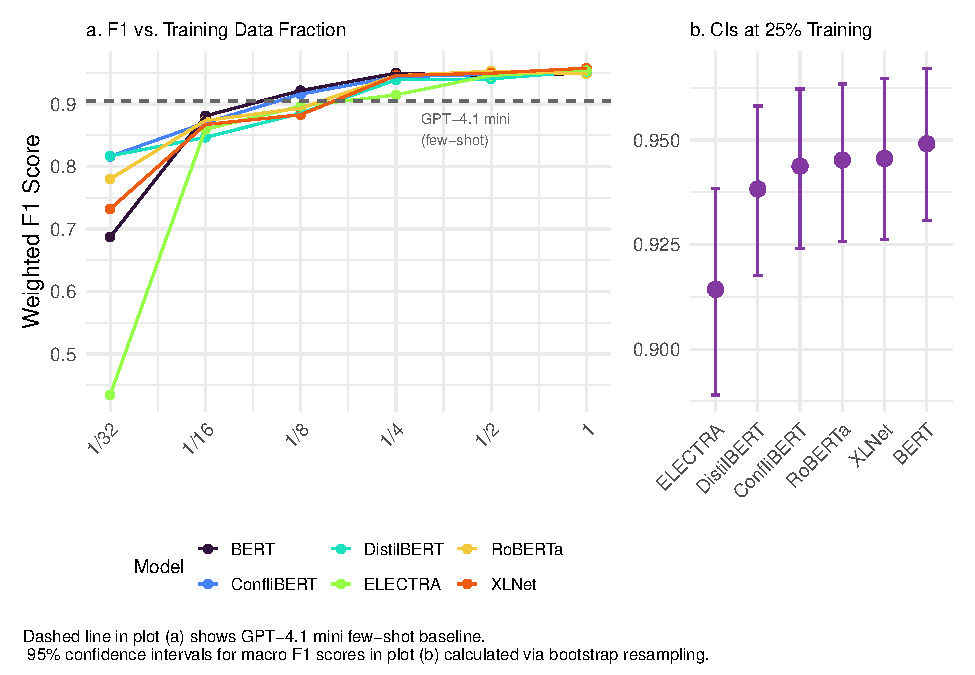
\includegraphics[keepaspectratio]{satp-classification_files/figure-pdf/perpetrator-1.pdf}}

}

\caption{Model Performance for `Perpetrator' Task}

\end{figure}%

The dashed line in Figure 1a marks the GPT-4.1 mini few-shot baseline,
which achieves a weighted F1 of 0.905 without any task-specific
fine-tuning. Every encoder model surpasses this level once trained on
roughly one-eighth of the labeled data, illustrating how quickly
fine-tuning closes and then widens the gap relative to prompting alone.

Consistent with findings reported in the original ConfliBERT paper
(\citeproc{ref-hu2022}{Hu et al. 2022}), we observe that ConfliBERT
performs particularly well at lower data fractions, where its
domain-specific pretraining appears to confer an advantage. However, the
gap narrows quickly. At the 1/8 training level, RoBERTa and XLNet both
achieve F1 scores that are not statistically distinguishable from
ConfliBERT's, perhaps complicating a straightforward narrative about
domain-specific model superiority (\citeproc{ref-brandt2024}{Brandt et
al. 2024}; \citeproc{ref-osorio2024}{Osorio et al. 2024}).

When trained on the full dataset, all models converge to very high
weighted macro F1 scores, ranging from 0.957 (ConfliBERT) to 0.968
(RoBERTa). This tight clustering in performance likely reflects the
relative simplicity of the classification task (predicting whether an
actor is Maoist, Security, or Other) and the benefit of high-quality,
consistent human annotations. While ConfliBERT retains a slight
advantage in low-resource settings, the results at full training suggest
that general-purpose encoder models are capable of matching or exceeding
the performance of domain-specific alternatives on this task. In a later
section, we return to inference speed and other performance trade-offs,
which further contextualize these results for applications in
low-resource environments.

\subsection{Action Type Task}\label{action-type-task}

The second task is a multi-label classification problem in which models
predict one or more action types associated with a given incident. These
include Armed Assault, Bombing, Abduction, Seizure, Arrest, Surrender,
and Facility/Infrastructure Attack. Performance is evaluated using micro
F1 scores, which are better suited to imbalanced, multi-label settings
where many samples carry multiple labels or none at all.

Figure 2a presents model performance across increasing training data
fractions, with the GPT-4.1 mini few-shot baseline shown as a dashed
line at 0.896. The decoder-only baseline performs well on this task,
achieving a competitive score without any fine-tuning. While encoders do
surpass it with sufficient training data, the margin at full training is
modest; the best encoder (XLNet, 0.939) exceeds the GPT baseline by only
a few points, suggesting that action type categories are distinctive
enough for a general-purpose model to classify from examples alone. Most
models cross the GPT baseline by the 12.5\% training fraction. As in the
perpetrator task, we observe notable variation in learning rates.
RoBERTa and XLNet clearly lead at the 25\% training level (Figure 2b),
with micro F1 scores of 0.882 and 0.879, respectively. ConfliBERT trails
modestly behind at 0.857, while BERT and DistilBERT cluster around 0.800
and 0.785. ELECTRA performs substantially worse, achieving a score of
only 0.636 at this level.

\begin{figure}[H]

{\centering \pandocbounded{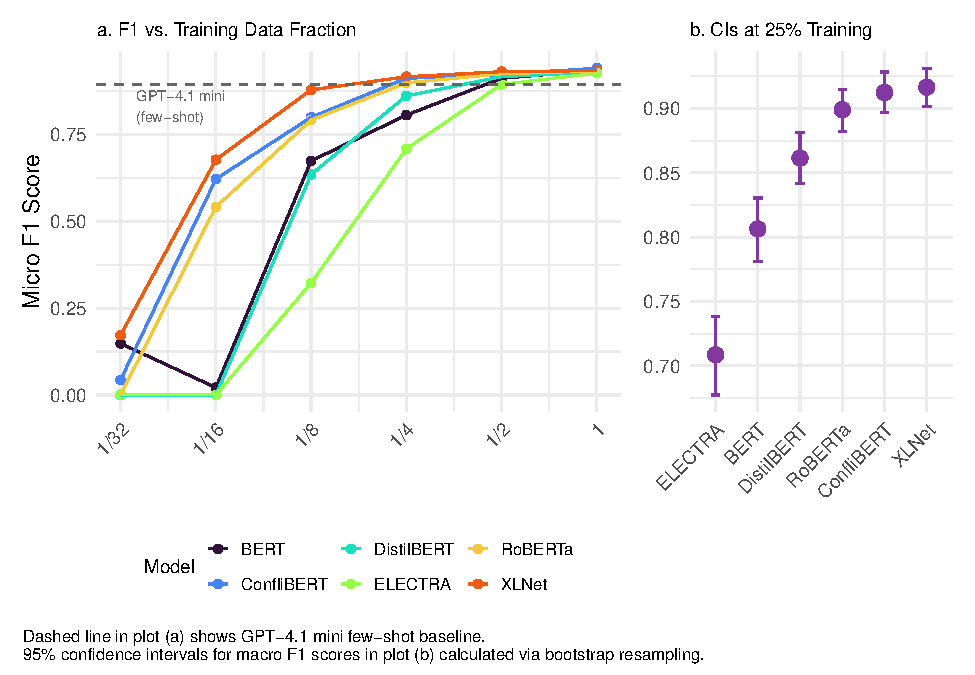
\includegraphics[keepaspectratio]{satp-classification_files/figure-pdf/action_type_performance-1.pdf}}

}

\caption{Model Performance for `Action Type' Task}

\end{figure}%

When trained on the full dataset, all models perform well, converging to
micro F1 scores in a narrow band between 0.915 (ELECTRA) and 0.939
(XLNet). The top four models (XLNet, RoBERTa, BERT, and ConfliBERT) are
separated by only a few hundredths of a point, underscoring a high level
of overall convergence. Once again, ConfliBERT performs strongly in
low-data regimes but is closely matched or outperformed by
general-purpose encoder models when more training data are available.

\begin{figure}[H]

{\centering \pandocbounded{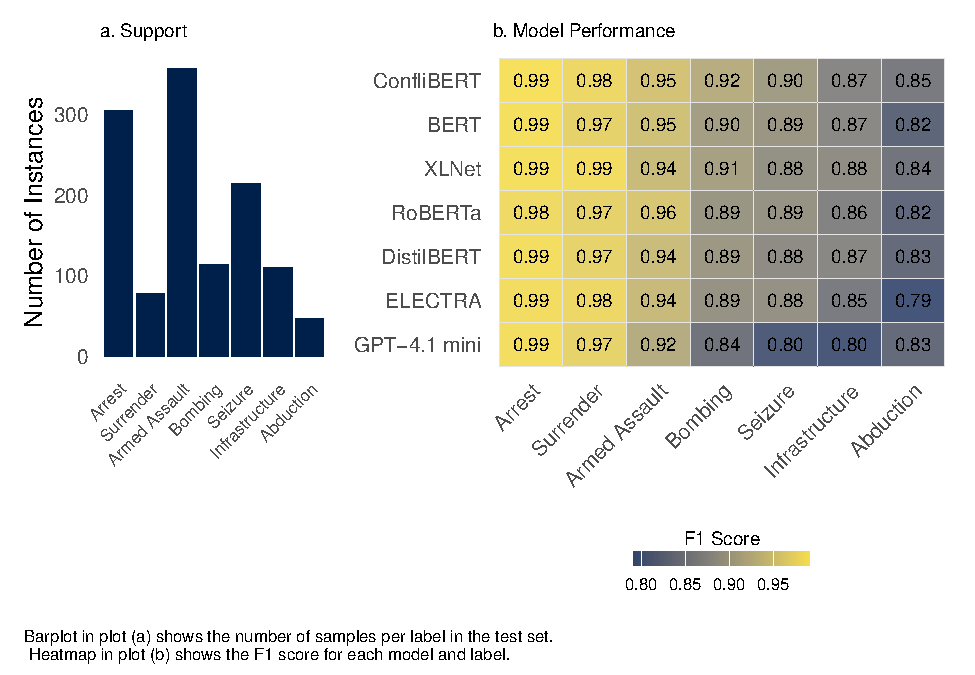
\includegraphics[keepaspectratio]{satp-classification_files/figure-pdf/action_type_labels-1.pdf}}

}

\caption{Model Performance by `Action Type' Label}

\end{figure}%

These headline results, however, mask important variation across action
types. As shown in Figure 3, which includes GPT-4.1 mini alongside the
encoder models, some labels (e.g., Surrender) are predicted with very
high accuracy despite low support in the training set, while others
(e.g., Facility/Infrastructure Attack) perform less well despite being
relatively more common. The GPT baseline shows a similar pattern: it
handles lexically distinctive categories well but struggles with labels
that require more nuanced contextual understanding. This suggests that
label frequency alone does not fully explain model performance. Certain
labels may benefit from linguistic distinctiveness. For example, the
word ``surrender'' appears with few synonyms or paraphrases in the
source texts, while others, like infrastructure-related actions, may
involve greater lexical ambiguity or more diverse expressions, making
them harder to classify.

\subsection{Target Type Task}\label{target-type-task}

The final task involves predicting one or more target types associated
with each incident. As in the action classification task, this is a
multi-label setting, and performance is again evaluated using micro F1
scores. Target categories include Security, Civilians, Officials,
Government Infrastructure, Private Property, Mining Companies, NGOs,
Other Groups, and Maoists.

Figure 4a presents model performance across training fractions. The
GPT-4.1 mini few-shot baseline (dashed line at 0.523) is notably lower
here than on the other two tasks, reflecting the greater difficulty of
target type classification for a model relying solely on in-context
examples. Figure 4b zooms into the 50\% training level, where we again
observe a clear performance cluster among XLNet, ConfliBERT, and
RoBERTa. At this level, XLNet leads with a micro F1 score of 0.839,
followed by ConfliBERT (0.819) and RoBERTa (0.816). DistilBERT and BERT
score considerably lower (0.770 and 0.710, respectively), and ELECTRA
again falls well behind the others at 0.614.

\begin{figure}[H]

{\centering \pandocbounded{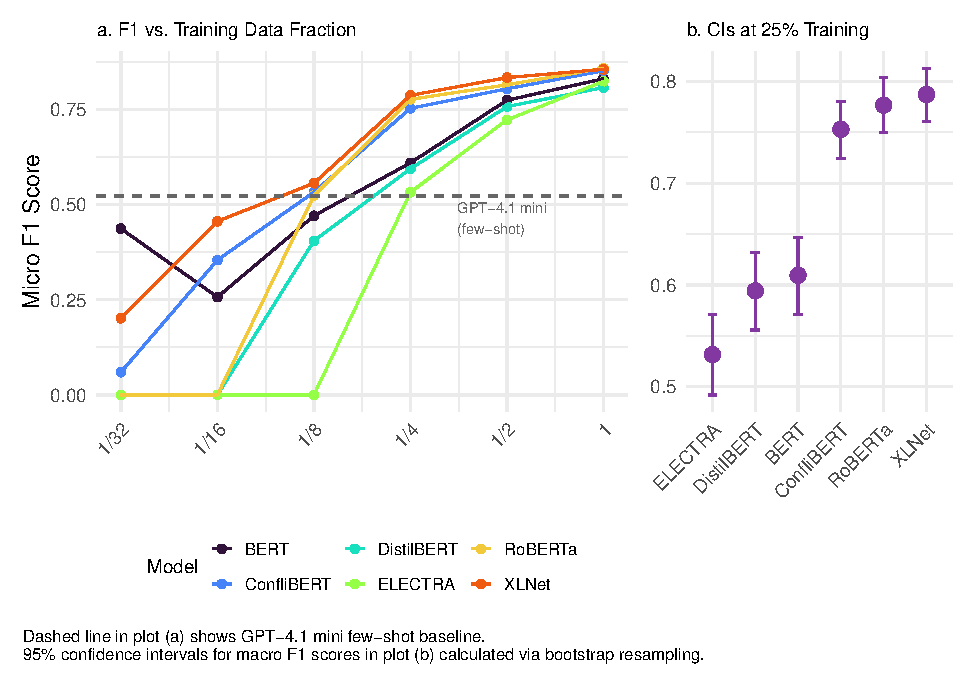
\includegraphics[keepaspectratio]{satp-classification_files/figure-pdf/target_type_performance-1.pdf}}

}

\caption{Model Performance for `Target Type' Task}

\end{figure}%

At full training (Figure 4a, rightmost points), model scores converge
somewhat, but still lag those observed in the action type task.
ConfliBERT reaches 0.878, with RoBERTa (0.870) and XLNet (0.869) close
behind. However, performance tails off for BERT (0.847), DistilBERT
(0.826), and ELECTRA (0.787). These figures indicate that target
prediction is a more difficult task overall, likely due to higher class
imbalance and greater semantic ambiguity in the expression of target
entities.

\begin{figure}[H]

{\centering \pandocbounded{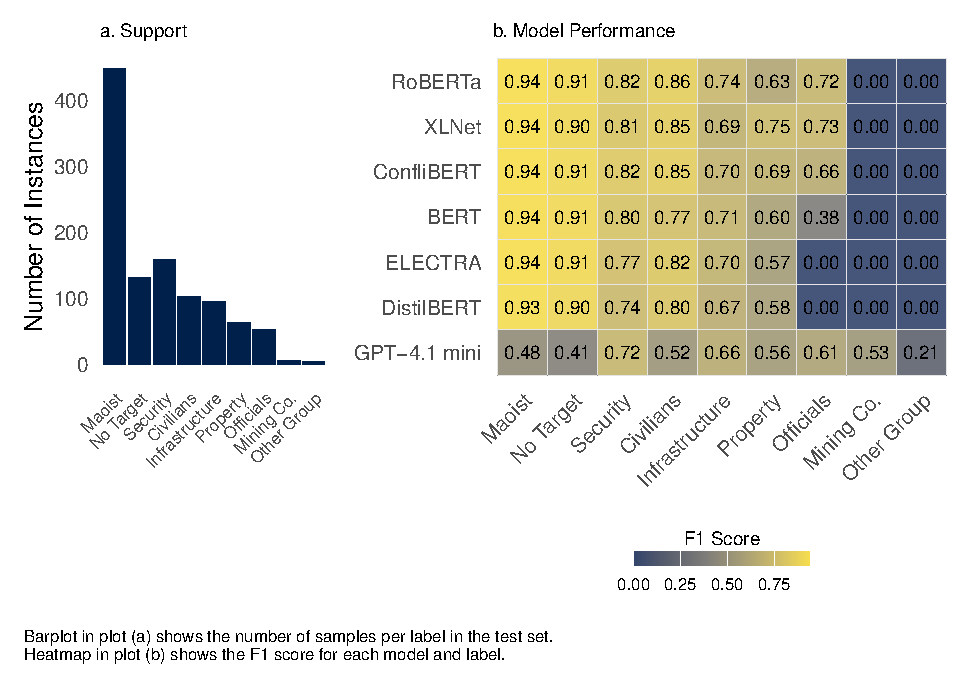
\includegraphics[keepaspectratio]{satp-classification_files/figure-pdf/target_type_labels-1.pdf}}

}

\caption{Model Performance by `Target Type' Label}

\end{figure}%

Figure 5 further illustrates this point by breaking down F1 scores
across individual labels. Some target types, particularly those with
limited support in the training set, show markedly lower performance.
However, the decline is not solely attributable to frequency. For
example, Surrender in the action task achieved strong scores despite low
support, likely due to its lexical distinctiveness. By contrast,
Infrastructure/Facility targets underperform even when relatively
frequent, suggesting that greater lexical variability and ambiguity in
how these targets are described contributes to model error.

\subsection{Performance-Speed
Tradeoffs}\label{performance-speed-tradeoffs}

Figure 6 presents a performance--speed comparison for the action and
target type classification tasks, plotting micro F1 scores against
evaluation speed (measured in samples per second). The figure highlights
the trade-offs between model accuracy and runtime efficiency, which are
especially relevant for researchers working in low-resource or
latency-sensitive environments.

\begin{figure}[H]

{\centering \pandocbounded{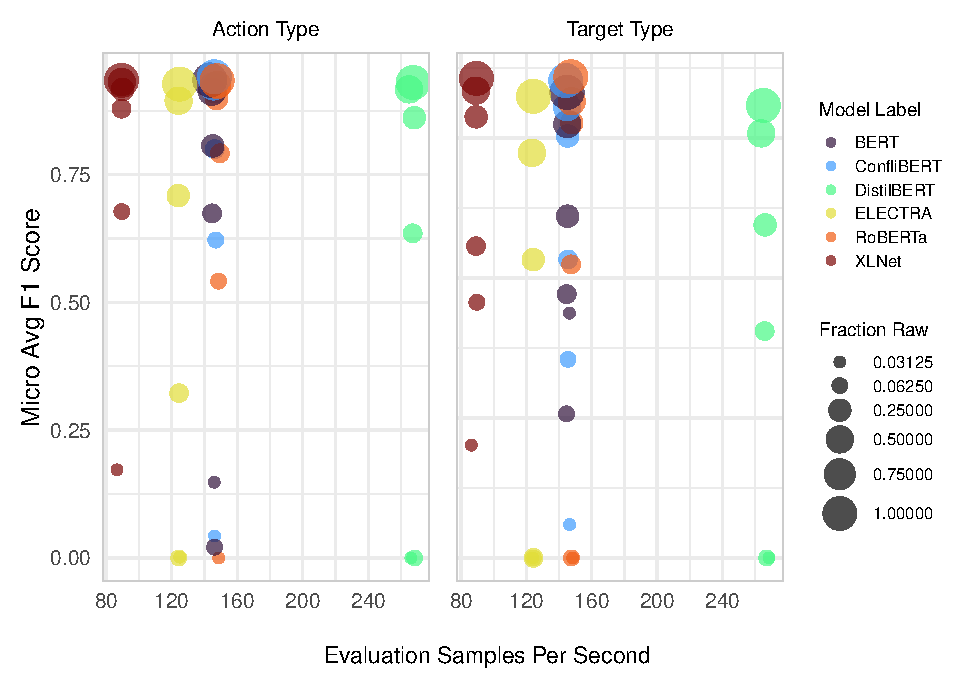
\includegraphics[keepaspectratio]{satp-classification_files/figure-pdf/performance_vs_speed-1.pdf}}

}

\caption{Model Performance vs.~Speed for Multiclass Classification
Tasks}

\end{figure}%

Among the top-performing models, RoBERTa and ConfliBERT stand out for
their efficiency. At full training, both achieve micro F1 scores near
the top of the range (0.870 and 0.878, respectively, on the target task)
while maintaining high evaluation speeds of 147 and 145 samples per
second. BERT, while slightly less performant (0.847), operates at a
comparable speed (144 samples/sec), making it a viable option where
pretraining data diversity is sufficient.

In contrast, XLNet, though highly competitive in terms of accuracy
(0.869), is much slower, evaluating at only 65 samples per second, less
than half the speed of RoBERTa and ConfliBERT. This substantial
performance-cost trade-off limits XLNet's practical appeal in
time-constrained settings.

DistilBERT emerges as the fastest model, running at 267 samples per
second, but as seen earlier, it tends to underperform at lower training
fractions, making it less suitable for small-data scenarios. ELECTRA
performs poorly on both axes: it is the least accurate model (0.787) and
also slower than most of its peers (124 samples/sec), suggesting limited
utility for either high-accuracy or speed-critical tasks.

Though Figure 6 focuses on the action and target type tasks, patterns
are similar for the perpetrator classification task (not shown). In all
cases, the results suggest that RoBERTa and ConfliBERT offer the best
balance between accuracy and efficiency, particularly when high
throughput is required alongside strong classification performance.

\section{Improving Low-Frequency Label
Performance}\label{improving-low-frequency-label-performance}

While our baseline encoder models demonstrated strong performance on
frequent target types such as ``Maoist,'' ``Security,'' and
``Civilians'', they exhibited complete failure on the rarest categories.
Specifically, models achieved zero F1 scores for ``Mining Company'' and
``Non-Maoist Armed Group'' across all six encoder architectures tested.
This pattern reflects the common challenge in conflict event
classification in that some of the most operationally significant events
such as those involving corporate targets or non-state armed actors
often represent the smallest fractions of training.

This class imbalance pattern, while not extreme, creates meaningful
challenges for classification performance. In our SATP training dataset,
``Mining Company'' targets comprise 54 instances (0.7\% of training
examples) while ``Non-Maoist Armed Group'' targets appear in 48
instances (0.6\% of training examples), compared to 3,583 ``Maoist''
examples (45.1\%) and 1,270 ``Civilian'' examples (16.0\%). Such
low-frequency labels create a challenging learning environment where
standard loss functions and sampling procedures struggle to develop
reliable decision boundaries.

\subsection{Imbalance Handling
Strategies}\label{imbalance-handling-strategies-1}

To systematically address these challenges, we implemented six distinct
imbalance handling strategies using ConfliBERT as our base model, each
targeting different aspects of the class imbalance problem through
modifications to loss functions, sampling procedures, or training data
augmentation. We selected ConfliBERT for this analysis given its strong
performance across the classification tasks explored earlier in this
paper and its domain-specific pretraining on conflict-related texts.

\textbf{Baseline Strategy.} Our baseline strategy provides a controlled
comparison using standard ConfliBERT training procedures with binary
cross-entropy loss and default 0.5 prediction thresholds. This baseline
leverages ConfliBERT's domain-specific representations while employing
conventional training approaches that struggle with class imbalance. All
experiments employed comprehensive reproducibility controls, including
fixed random seeds (42) across Python, NumPy, PyTorch, and CUDA
operations to ensure reliable comparisons across strategies.

\textbf{Threshold Tuning.} We tested threshold tuning both as a
standalone imbalance handling strategy and integrated it into the five
subsequent strategies explored below. As a standalone strategy,
threshold tuning represents a computationally efficient strategy
requiring no model retraining and therefore serves as an important
first-line approach for addressing class imbalance in operational
settings. We use macro PR-AUC for checkpoint selection during training
to ensure good representations across all classes before applying
post-training calibration and threshold optimization. The threshold
optimization process then starts with temperature scaling applied to
model outputs to improve probability calibration
(\citeproc{ref-guo2017}{Guo et al. 2017}), followed by grid search
optimization across threshold values from 0.05 to 0.95 (19 points) to
maximize micro-F1 performance on the validation set.

\textbf{Class Weights.} This traditional approach employs inverse
frequency weighting within the loss function, computing
\(\text{weight} = N_{\text{negative}}/N_{\text{positive}}\) for each
label and applying these weights via PyTorch's BCEWithLogitsLoss
(\citeproc{ref-he2009}{He and Garcia 2009}). This conceptually simply
method provides a strong baseline for comparison with more sophisticated
approaches.

\textbf{Weighted Sampling.} The weighted sampling strategy balances
training batches through strategic oversampling of underrepresented
examples using PyTorch's WeightedRandomSampler
(\citeproc{ref-buda2018}{Buda, Maki, and Mazurowski 2018}). Sample
weights are computed as 1 / (label\_count + 1), where label\_count
represents the sum of positive labels per example. This ensures that
rare examples appear multiple times per epoch while enabling replacement
sampling to maintain batch diversity.

\textbf{Focal Loss.} The focal loss strategy addresses class imbalance
through a modified loss function that dynamically focuses learning on
hard-to-classify examples (\citeproc{ref-lin2018}{Lin et al. 2018}). We
replaced standard binary cross-entropy with focal loss using
automatically computed per-label alpha weights:

\[\alpha_{\text{pos}} = \text{clamp}\left(\sqrt{\frac{\text{median prevalence}}{\text{label prevalence}}}, 0.25, 0.75\right)\]

where \emph{median\_prevalence} represents the typical frequency across
all target types in our dataset, \emph{label\_prevalence} is the
frequency of the specific target type being weighted, and \emph{clamp}
constrains the resulting weight to fall between 0.25 and 0.75 to ensure
training stability. This formulation automatically assigns higher
weights to rare labels like ``Mining Company'' (0.7\% prevalence) while
reducing weights for common labels like ``Maoist'' (45.1\% prevalence).
The gamma parameter was set to 2.0 for standard imbalanced labels and
boosted to 2.5 for ultra-rare labels (prevalence \textless{} 1\%). This
adaptive parameterization eliminates manual hyperparameter tuning while
ensuring appropriate focus on the most challenging examples.

\textbf{Back-Translation Augmentation.} Our back-translation strategy
generates synthetic training examples for underrepresented categories
through translation-based paraphrasing
(\citeproc{ref-sennrich2016}{Sennrich, Haddow, and Birch 2016};
\citeproc{ref-halterman2025}{Halterman 2025}). We employed an automatic
threshold-based approach, targeting all labels with fewer than 900
positive training examples to systematically address imbalance across
``Mining Company'' (54 training examples), ``Non-Maoist Armed Group''
(48 examples), ``Private Property'' (509 examples), and ``Government
Infrastructure'' (771 examples). The strategy translates English
incident summaries through Hindi, Urdu, and Bengali, languages
contextually relevant to South Asian conflict data, before
back-translating to English using Google Translate API. Synthetic
generation was constrained by safety parameters: a maximum of 500 new
examples per label and a synthesis ratio preventing synthetic examples
from exceeding original positive counts. The strategy preferentially
selects single-label positive examples to minimize label co-occurrence
artifacts, effectively doubling training data for the most
underrepresented categories while providing controlled expansion for
moderately imbalanced labels.

\textbf{T5 Paraphrase Augmentation.} This strategy employs Google
FLAN-T5-Large for high-quality paraphrase generation under identical
threshold-based selection criteria and safety constraints as
back-translation (\citeproc{ref-chung2022}{Chung et al. 2022};
\citeproc{ref-parolin2022b}{Parolin et al. 2022}). The approach uses
structured prompts emphasizing factual preservation and neutral tone,
with quality control through similarity filtering using
sentence-transformers (all-MiniLM-L6-v2), accepting paraphrases with
cosine similarity between 0.85-0.98 to original text. Generation
parameters (temperature=0.7, top\_p=0.9) ensure semantic consistency
while creating meaningful variation. The same label selection and
synthesis ratio constraints as back-translation are applied to achieve a
balanced augmentation strategy that enhances representation for rare
categories without overwhelming the original data distribution.

\subsection{Improvements on Low-Frequency
Categories}\label{improvements-on-low-frequency-categories}

Our imbalance handling strategies achieved transformative improvements
on previously unlearnable categories, as illustrated in Figure 7. For
example, ``Mining Company'' targets improved from complete failure (0.00
F1) across all baseline models to substantial performance under weighted
sampling (0.625 F1), while ``Non-Maoist Armed Group'' targets reached
0.857 F1 using back-translation augmentation, representing infinite
relative improvement over baseline performance.

\begin{figure}[H]

{\centering \pandocbounded{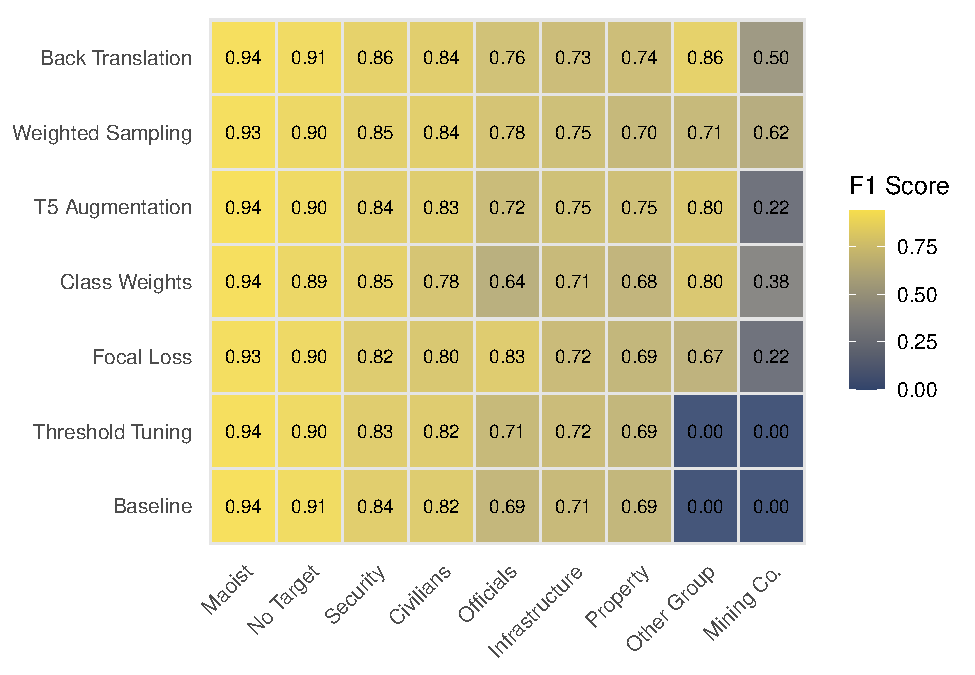
\includegraphics[keepaspectratio]{satp-classification_files/figure-pdf/imbalance-handling-heatmap-1.pdf}}

}

\caption{Performance of Six Imbalance Handling Strategies}

\end{figure}%

The heatmap reveals distinct strategy profiles across the target type
spectrum. Back translation augmentation emerged as the most consistently
effective approach, achieving strong performance across both rare
categories (Mining Company: 0.50, Non-Maoist Armed Group: 0.857). T5
augmentation demonstrated comparable effectiveness with particularly
strong performance on ``Government Infrastructure'' (0.751) and
``Private Property'' (0.748) targets.

Weighted sampling showed remarkable effectiveness for ``Mining Company''
targets (0.625 F1) and solid performance on ``Civilians'' (0.842),
suggesting that oversampling strategies may be particularly valuable for
targets with moderate scarcity. Class weights and focal loss provided
meaningful but more modest improvements, while threshold tuning alone,
despite sophisticated optimization, failed to overcome the fundamental
learning challenges posed by extreme class imbalance.

Crucially, these improvements on rare categories were attained without
degrading performance on frequent targets. All strategies maintained
strong F1 scores above 0.82 for ``Security,'' ``Civilians,'' and
``Maoist'' categories, indicating that the approaches successfully
addressed imbalance without creating negative transfer effects.

\subsection{Precision-Recall Tradeoffs in Rare Category
Classification}\label{precision-recall-tradeoffs-in-rare-category-classification}

The precision-recall plots for our four target rare categories (Figure
8) illuminate the distinct approaches each strategy takes to the
precision-recall optimization problem. These plots reveal that achieving
high performance on rare categories requires navigating fundamental
tradeoffs between conservative precision and comprehensive recall, with
different strategies occupying distinct regions of the precision-recall
space.

\begin{figure}[H]

{\centering \pandocbounded{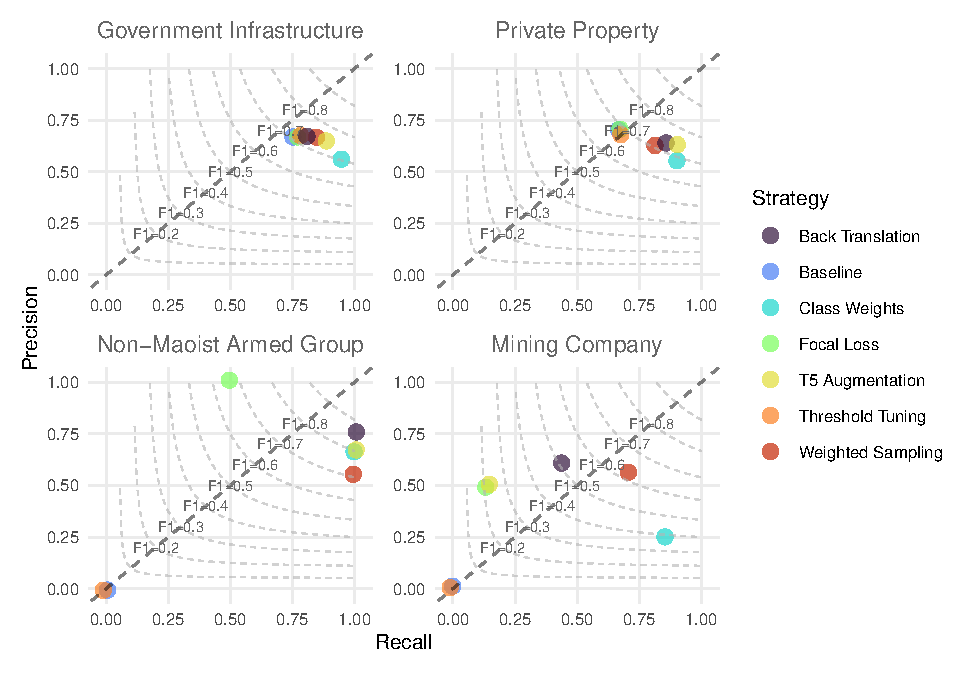
\includegraphics[keepaspectratio]{satp-classification_files/figure-pdf/PR plots-1.pdf}}

}

\caption{Precision-Recall Plots for Imbalance Handling Strategies}

\end{figure}%

Back-translation augmentation consistently achieves the highest F1
scores (0.72-0.76) across rare categories through well-balanced
precision-recall profiles. This balanced approach suggests that
high-quality synthetic examples enable models to develop robust decision
boundaries that perform reliably across both precision and recall
dimensions.

Focal loss demonstrates a precision-specialist profile, garnering
perfect precision (1.0) for ``Non-Maoist Armed Group'' classification
while sacrificing recall (\textasciitilde0.5). This pattern aligns with
focal loss's theoretical foundation of focusing learning on the hardest
examples, and in doing so the model becomes highly conservative but
accurate in its positive predictions. This precision-emphasis may be
operationally valuable in applications where false positives carry high
analytical costs.

Weighted sampling and class weights occupy intermediate positions,
suggesting these approaches provide reasonable compromises between
precision and recall without strongly favoring either dimension. T5
augmentation shows solid, consistent performance across categories,
typically achieving good precision-recall balance albeit with slightly
lower overall F1 scores than back-translation.

These precision-recall profiles have important implications for
operational deployment. High-precision strategies like focal loss may be
preferred when human analysts must review flagged events, as they
minimize false positive rates that could overwhelm analytical capacity.
Conversely, high-recall approaches may be more appropriate for
comprehensive monitoring applications where missing true events carries
greater costs than processing false positives. The balanced profiles
achieved by augmentation strategies suggest they may be most suitable
for general-purpose classification where both precision and recall
matter equally.

\section{Conclusion}\label{conclusion}

This study evaluated six encoder-based transformer architectures and one
generative GPT model on three classification tasks drawn from the South
Asia Terrorism Portal: perpetrator attribution, action type, and target
type. Across tasks, fine-tuned encoders achieved strong performance on
high-frequency labels even at small data fractions, while low-frequency
labels remained challenging until addressed with targeted
imbalance-handling strategies. Back-translation through contextually
relevant languages proved somewhat effective in classifying previously
unlearnable categories.

The GPT-4.1 mini few-shot baselines add a practical reference point. On
perpetrator classification, a single-label task with three
well-separated categories, GPT-4.1 mini achieved competitive F1 with
zero labeled training data. On action type it performed respectably,
though fine-tuned encoders surpassed it once trained on roughly
one-eighth of the available data. On target type, where the taxonomy is
more granular and the label space larger, the few-shot generative
approach struggled considerably. These results suggest that the amount
of labor NLP tools can save depends heavily on task structure.

For researchers deciding how to invest their time, these findings imply
a practical decision tree. When a classification task involves a small
number of well-defined categories, a generative model with a carefully
constructed prompt may be sufficient out of the box, requiring no
labeled data at all. When the taxonomy is more complex or the generative
baseline falls short, the results here show that fine-tuned encoders
overtake GPT baselines with relatively modest annotation efforts,
roughly on the order of one thousand labeled examples rather than tens
of thousands. The traditional assumption that automated coding requires
massive hand-coded training sets no longer holds. Even a targeted,
limited annotation campaign can yield a classifier that outperforms both
manual scaling and zero-shot generative approaches.

A related question that the field rarely confronts directly is what
level of automated classification performance justifies replacing human
coders. The implicit standard is that higher accuracy is always better,
but human inter-coder reliability is itself imperfect. Major conflict
datasets disagree at non-trivial rates on event classification for the
same conflicts (\citeproc{ref-eck2012}{Eck 2012}). The appropriate
benchmark for automated systems may not be perfection but parity with
trained human coders on equivalent tasks. Researchers should consider
what level of classification error is tolerable for their downstream
analysis, particularly in light of evidence that treating predicted
labels as error-free biases parameter estimates even when classification
accuracy exceeds 90 percent (\citeproc{ref-egami2024}{Egami et al.
2024}).

Even with these methodological advances, adoption is not frictionless.
Most political scientists are trained in inferential statistics and R,
while the NLP tools evaluated here originate from data science and are
implemented in Python. Generative AI lowers the entry barrier in that
prompting a model requires no machine learning expertise, but
fine-tuning workflows still carry a learning curve. Funding remains a
necessity: for annotation (even if smaller-scale than previously
assumed), for computational resources, and for methodological training.
The history of abandoned or defunded coding projects illustrates what
happens when event-data infrastructure depends on continuous grant
support (\citeproc{ref-nardulli2015}{Nardulli, Althaus, and Hayes 2015};
\citeproc{ref-croicu2015}{Croicu and Weidmann 2015}). Sustainable
adoption requires not just better models but institutional commitments
to maintaining them.

Researchers working with sensitive conflict data face an additional
constraint. Commercial generative APIs require transmitting text,
potentially containing information about informants, ongoing operations,
or vulnerable populations, to third-party servers. Open-source encoder
models that can be fine-tuned and deployed locally address these
data-sovereignty concerns in ways that cloud-based generative services
cannot (\citeproc{ref-weber2023}{Weber and Reichardt 2023};
\citeproc{ref-grossmann2023}{Grossmann et al. 2023}). This consideration
may tip the build-versus-buy calculus toward fine-tuned models even when
generative baselines achieve acceptable accuracy.

Looking ahead, the most promising direction may be hybrid pipelines that
combine the strengths of both paradigms, employing generative models for
rapid prototyping and initial labeling, followed by fine-tuned encoders
with requisite imbalance handling for production deployment where speed,
cost, privacy, or accuracy on complex taxonomies demand it. As both
model families continue to improve, the practical question for conflict
researchers is shifting from whether automated coding is viable to how
best to integrate it into existing research workflows.

\newpage

\section{Appendix}\label{appendix}

\subsection{A1. Decoder-Only LLM Baseline
Results}\label{sec-llm-results}

Table~\ref{tbl-llm-comparison} presents the full results of zero-shot
and few-shot classification using three decoder-only LLMs: GPT-4o-mini,
GPT-4.1 mini, and GPT-5.2. These models were evaluated on the same test
sets used for the encoder-based models. GPT-4.1 mini few-shot achieved
the best overall performance among the decoder-only models and is used
as the baseline reference in Figures 1--5.

\begin{longtable}[]{@{}
  >{\raggedright\arraybackslash}p{(\linewidth - 10\tabcolsep) * \real{0.1739}}
  >{\raggedright\arraybackslash}p{(\linewidth - 10\tabcolsep) * \real{0.1884}}
  >{\centering\arraybackslash}p{(\linewidth - 10\tabcolsep) * \real{0.1594}}
  >{\centering\arraybackslash}p{(\linewidth - 10\tabcolsep) * \real{0.1449}}
  >{\centering\arraybackslash}p{(\linewidth - 10\tabcolsep) * \real{0.1449}}
  >{\centering\arraybackslash}p{(\linewidth - 10\tabcolsep) * \real{0.1884}}@{}}

\caption{\label{tbl-llm-comparison}Decoder-Only LLM Classification
Results (Zero-Shot and Few-Shot)}

\tabularnewline

\toprule\noalign{}
\begin{minipage}[b]{\linewidth}\raggedright
Task
\end{minipage} & \begin{minipage}[b]{\linewidth}\raggedright
Model
\end{minipage} & \begin{minipage}[b]{\linewidth}\centering
Mode
\end{minipage} & \begin{minipage}[b]{\linewidth}\centering
Micro F1
\end{minipage} & \begin{minipage}[b]{\linewidth}\centering
Macro F1
\end{minipage} & \begin{minipage}[b]{\linewidth}\centering
Weighted F1
\end{minipage} \\
\midrule\noalign{}
\endhead
\bottomrule\noalign{}
\endlastfoot
Perpetrator & GPT-4o-mini & Zero-shot & 0.819 & 0.605 & 0.811 \\
Perpetrator & GPT-4o-mini & Few-shot & 0.829 & 0.680 & 0.837 \\
Action Type & GPT-4o-mini & Zero-shot & 0.857 & 0.825 & 0.867 \\
Action Type & GPT-4o-mini & Few-shot & 0.892 & 0.876 & 0.897 \\
Target Type & GPT-4o-mini & Zero-shot & 0.541 & 0.523 & 0.589 \\
Target Type & GPT-4o-mini & Few-shot & 0.515 & 0.508 & 0.541 \\
Perpetrator & GPT-4.1-mini & Zero-shot & 0.880 & 0.679 & 0.872 \\
Perpetrator & GPT-4.1-mini & Few-shot & 0.899 & 0.783 & 0.905 \\
Action Type & GPT-4.1-mini & Zero-shot & 0.893 & 0.882 & 0.895 \\
Action Type & GPT-4.1-mini & Few-shot & 0.896 & 0.878 & 0.898 \\
Target Type & GPT-4.1-mini & Zero-shot & 0.655 & 0.576 & 0.678 \\
Target Type & GPT-4.1-mini & Few-shot & 0.523 & 0.521 & 0.535 \\
Perpetrator & GPT-5.2 & Zero-shot & 0.889 & 0.715 & 0.884 \\
Perpetrator & GPT-5.2 & Few-shot & 0.883 & 0.759 & 0.882 \\
Action Type & GPT-5.2 & Zero-shot & 0.893 & 0.870 & 0.898 \\
Action Type & GPT-5.2 & Few-shot & 0.910 & 0.889 & 0.914 \\
Target Type & GPT-5.2 & Zero-shot & 0.628 & 0.551 & 0.699 \\
Target Type & GPT-5.2 & Few-shot & 0.627 & 0.560 & 0.653 \\

\end{longtable}

\newpage

\subsection{A2. Few-Shot Prompts}\label{sec-prompts}

For each task, the decoder-only models received a system prompt defining
the classification categories and a user prompt presenting the incident
text. In the few-shot condition, labeled examples were inserted as
user--assistant turn pairs before the test instance. The full prompts
and examples are reproduced below.

\subsubsection{Perpetrator Task}\label{perpetrator-task-1}

\textbf{System prompt:}

\begin{quote}
You are classifying conflict events from India's Maoist insurgency.
Given an event description, identify the perpetrator/action-taker.

Categories:

\begin{itemize}
\tightlist
\item
  Maoist: Maoist insurgents, Naxalites, or affiliated groups
\item
  Security: Government security forces, police, CRPF, military
\item
  Unknown: Cannot be determined from the text
\end{itemize}
\end{quote}

\textbf{User prompt template:}

\begin{quote}
Event: \{text\}

Respond with only one word: Maoist, Security, or Unknown
\end{quote}

\textbf{Few-shot examples (3):}

\begin{enumerate}
\def\labelenumi{\arabic{enumi}.}
\tightlist
\item
  ``Maoists killed Constable Krishnalal Dhurtlahare in Dantewada
  District.'' → \textbf{Maoist}
\item
  ``Acting on a tip off, Police arrested a CPI-Maoist cadre, identified
  as Bhola Ram, from Basata village under Telpa Police Station limits in
  Arwal District.'' → \textbf{Security}
\item
  ``Bokaro Police and the CRPF troopers were engaged in an encounter
  with the CPI-Maoist cadres at Kanshidih forest area in Jhumra under
  Gomia Police Station of Bokaro District.'' → \textbf{Unknown}
\end{enumerate}

\subsubsection{Action Type Task}\label{action-type-task-1}

\textbf{System prompt:}

\begin{quote}
You are classifying conflict events. An event may involve multiple
action types.

Categories:

\begin{itemize}
\tightlist
\item
  Armed Assault: Armed attacks, shootings, ambushes, firefights
\item
  Arrest: Detention, capture, apprehension by authorities
\item
  Bombing: Explosions, IEDs, landmines, blasts
\item
  Infrastructure: Attacks on facilities, sabotage, arson of buildings
\item
  Surrender: Voluntary surrender, laying down arms
\item
  Seizure: Raids, confiscation of weapons/materials
\item
  Abduction: Kidnapping, hostage-taking
\end{itemize}
\end{quote}

\textbf{User prompt template:}

\begin{quote}
Event: \{text\}

List all applicable categories, separated by commas. If none apply
clearly, respond ``None''.
\end{quote}

\textbf{Few-shot examples (5):}

\begin{enumerate}
\def\labelenumi{\arabic{enumi}.}
\tightlist
\item
  ``CPI-Maoist cadres shot dead a leader of the Congress party, Shaik
  Sabakthulla, at Madithadu village in the Cuddapah District.'' →
  \textbf{Armed Assault}
\item
  ``Three Maoists surrendered before the Police in Dornapal town of
  Sukma District.'' → \textbf{Surrender}
\item
  ``Two CRPF troopers were killed and three others were injured when
  Maoists triggered an explosive, when they were on way to a polling
  station in Jamui District parliamentary constituency.'' →
  \textbf{Bombing}
\item
  ``Three cadres of the PLFI, a breakaway faction of the CPI-Maoist,
  including an `area commander', were arrested from Dhodhtritoli under
  Raidih Police Station in Gumla District. Gumla SP Jatin Narwal said
  the arrested PLFI cadres have been identified as `area commander'
  Durjan Singh, Surendra Pal Singh and Bandhan Oraon - all residents of
  the same Police Station areas of the District. `Police recovered a
  country-made pistol, eight sim cards, a cell phone and four live
  bullets besides a dairy containing names of the persons from whom PLFI
  activists extorted levy,' said the SP.'' → \textbf{Arrest, Seizure}
\item
  ``Three abducted Policemen, identified as Lakhan Netam, Chandrasekhar
  Thakur and Ramprakahs Tiwari of Amabeda Police Station, were released
  by the CPI-Maoist in the Kanker District. The released Policemen said
  they were abducted when they had gone to Sode village under Amabeda
  Police Station to make telephone calls to their homes. The extremists
  also took their mobile handsets and two motor cycles. According to the
  Police, the Maoists had taken them deep into the forest, tied them to
  trees and threatened them to quit the Police service.'' →
  \textbf{Abduction}
\end{enumerate}

\subsubsection{Target Type Task}\label{target-type-task-1}

\textbf{System prompt:}

\begin{quote}
You are classifying the targets of conflict events. An event may have
multiple targets.

Categories:

\begin{itemize}
\tightlist
\item
  Maoist: Maoist insurgents or their camps/facilities
\item
  Security: Police, military, paramilitary forces
\item
  Civilians: Non-combatant individuals
\item
  Government Officials: Politicians, bureaucrats, elected officials
\item
  Government Infrastructure: Government buildings, roads, bridges,
  railways
\item
  Private Property: Civilian homes, businesses, vehicles
\item
  Mining Company: Mining operations, personnel, or equipment
\item
  Non-Maoist Armed Group: Other armed groups (not Maoist or government)
\item
  No Target: No specific target (e.g., surrenders)
\end{itemize}
\end{quote}

\textbf{User prompt template:}

\begin{quote}
Event: \{text\}

List all applicable categories, separated by commas.
\end{quote}

\textbf{Few-shot examples (5):}

\begin{enumerate}
\def\labelenumi{\arabic{enumi}.}
\tightlist
\item
  ``One CRPF trooper was injured when CPI-Maoist cadres triggered a
  series of landmines targeting the SF personnel on a combing operation
  in Rudakota area'' → \textbf{Security}
\item
  ``A husband and wife duo, Durjodhan Rajkowar and his wife Lalita,
  members of a Maoist squad operating in the Ayodhya Hills of Purulia
  District surrendered before the District Police.'' → \textbf{No
  Target}
\item
  ``CPI-Maoist cadres blew up a newly constructed health sub-centre
  building in Serendag village under Herhanj Police Station in Latehar
  District.'' → \textbf{Government Infrastructure}
\item
  ``A civilian and 11 Policeman were killed and three sustained injuries
  in an ambush set by the CPI-Maoist cadres in Metlaperu village forests
  under Bhadrakali Police Station area of Bijapur District.'' →
  \textbf{Civilians, Security}
\item
  ``About 150 cadres of the CPI-Maoist raided a stone-mine in Bastar
  region for explosives. However, when they could not find any
  explosive, they set ablaze eight stone crusher machines at Partha and
  Darbha areas of the region.'' → \textbf{Mining Company}
\end{enumerate}

\newpage

\section{References}\label{references}

\setlength{\parindent}{-0.2in}
\setlength{\leftskip}{0.2in}
\setlength{\parskip}{8pt}
\noindent

\phantomsection\label{refs}
\begin{CSLReferences}{1}{0}
\bibitem[\citeproctext]{ref-abdurahman2025}
Abdurahman, Suhaib, Alireza Salkhordeh Ziabari, Alexander K. Moore,
Daniel M. Bartels, and Morteza Dehghani. 2025. {``A {Primer} for
{Evaluating Large Language Models} in {Social-Science Research}.''}
\emph{Advances in Methods and Practices in Psychological Science} 8 (2):
25152459251325174. \url{https://doi.org/10.1177/25152459251325174}.

\bibitem[\citeproctext]{ref-brandt2025}
Brandt, Patrick T., Sultan Alsarra, Vito D'Orazio, Dagmar Heintze,
Latifur Khan, Shreyas Meher, Javier Osorio, and Marcus Sianan. 2025.
{``Extractive Versus {Generative Language Models} for {Political
Conflict Text Classification}.''} \emph{Political Analysis}, December,
1--29. \url{https://doi.org/10.1017/pan.2025.10027}.

\bibitem[\citeproctext]{ref-brandt2024}
Brandt, Patrick T., Sultan Alsarra, Vito J. D`Orazio, Dagmar Heintze,
Latifur Khan, Shreyas Meher, Javier Osorio, and Marcus Sianan. 2024.
{``{ConfliBERT}: {A Language Model} for {Political Conflict}.''}
December 19, 2024. \url{https://doi.org/10.48550/arXiv.2412.15060}.

\bibitem[\citeproctext]{ref-brown2020}
Brown, Tom B., Benjamin Mann, Nick Ryder, Melanie Subbiah, Jared Kaplan,
Prafulla Dhariwal, Arvind Neelakantan, et al. 2020. {``Language {Models}
Are {Few-Shot Learners}.''} July 22, 2020.
\url{https://doi.org/10.48550/arXiv.2005.14165}.

\bibitem[\citeproctext]{ref-buda2018}
Buda, Mateusz, Atsuto Maki, and Maciej A. Mazurowski. 2018. {``A
Systematic Study of the Class Imbalance Problem in Convolutional Neural
Networks.''} \emph{Neural Networks} 106 (October): 249--59.
\url{https://doi.org/10.1016/j.neunet.2018.07.011}.

\bibitem[\citeproctext]{ref-chung2022}
Chung, Hyung Won, Le Hou, Shayne Longpre, Barret Zoph, Yi Tay, William
Fedus, Yunxuan Li, et al. 2022. {``Scaling {Instruction-Finetuned
Language Models}.''} December 6, 2022.
\url{https://doi.org/10.48550/arXiv.2210.11416}.

\bibitem[\citeproctext]{ref-clark2020}
Clark, Kevin, Minh-Thang Luong, Quoc V. Le, and Christopher D. Manning.
2020. {``{ELECTRA}: {Pre-training Text Encoders} as {Discriminators
Rather Than Generators}.''} March 23, 2020.
\url{https://doi.org/10.48550/arXiv.2003.10555}.

\bibitem[\citeproctext]{ref-croicu2015}
Croicu, Mihai, and Nils B Weidmann. 2015. {``Improving the Selection of
News Reports for Event Coding Using Ensemble Classification.''}
\emph{Research \& Politics} 2 (4): 2053168015615596.
\url{https://doi.org/10.1177/2053168015615596}.

\bibitem[\citeproctext]{ref-devlin2019}
Devlin, Jacob, Ming-Wei Chang, Kenton Lee, and Kristina Toutanova. 2019.
{``{BERT}: {Pre-training} of {Deep Bidirectional Transformers} for
{Language Understanding}.''} In \emph{Proceedings of the 2019
{Conference} of the {North}}, 4171--86. Minneapolis, Minnesota:
Association for Computational Linguistics.
\url{https://doi.org/10.18653/v1/N19-1423}.

\bibitem[\citeproctext]{ref-eck2012}
Eck, Kristine. 2012. {``In Data We Trust? {A} Comparison of {UCDP GED}
and {ACLED} Conflict Events Datasets.''} \emph{Cooperation and Conflict}
47 (1): 124--41. \url{https://doi.org/10.1177/0010836711434463}.

\bibitem[\citeproctext]{ref-egami2024}
Egami, Naoki, Musashi Hinck, Brandon M Stewart, and Hanying Wei. 2024.
{``Using {Large Language Model Annotations} for the {Social Sciences}:
{A General Framework} of {Using Predicted Variables} in {Downstream
Analyses}.''}

\bibitem[\citeproctext]{ref-fetzer2020}
Fetzer, Thiemo. 2020. {``Can {Workfare Programs Moderate Conflict}?
{Evidence} from {India}.''} \emph{Journal of the European Economic
Association} 18 (6): 3337--75.
\url{https://doi.org/10.1093/jeea/jvz062}.

\bibitem[\citeproctext]{ref-ghatak2017a}
Ghatak, Maitreesh, and Oliver Vanden Eynde. 2017. {``Economic
{Determinants} of the {Maoist Conflict} in {India},''} no. 39.

\bibitem[\citeproctext]{ref-gilardi2023}
Gilardi, Fabrizio, Meysam Alizadeh, and Maël Kubli. 2023. {``{ChatGPT}
Outperforms Crowd Workers for Text-Annotation Tasks.''}
\emph{Proceedings of the National Academy of Sciences} 120 (30):
e2305016120. \url{https://doi.org/10.1073/pnas.2305016120}.

\bibitem[\citeproctext]{ref-grossmann2023}
Grossmann, Igor, Matthew Feinberg, Dawn C. Parker, Nicholas A.
Christakis, Philip E. Tetlock, and William A. Cunningham. 2023. {``{AI}
and the Transformation of Social Science Research.''} \emph{Science} 380
(6650): 1108--9. \url{https://doi.org/10.1126/science.adi1778}.

\bibitem[\citeproctext]{ref-guo2017}
Guo, Chuan, Geoff Pleiss, Yu Sun, and Kilian Q. Weinberger. 2017. {``On
{Calibration} of {Modern Neural Networks}.''} August 3, 2017.
\url{https://doi.org/10.48550/arXiv.1706.04599}.

\bibitem[\citeproctext]{ref-halterman2025}
Halterman, Andrew. 2025. {``Synthetically Generated Text for Supervised
Text Analysis.''} \emph{Political Analysis}, January, 1--14.
\url{https://doi.org/10.1017/pan.2024.31}.

\bibitem[\citeproctext]{ref-halterman2021}
Halterman, Andrew, Katherine Keith, Sheikh Sarwar, and Brendan O'Connor.
2021. {``Corpus-{Level Evaluation} for {Event QA}: {The
IndiaPoliceEvents Corpus Covering} the 2002 {Gujarat Violence}.''} In
\emph{Findings of the {Association} for {Computational Linguistics}:
{ACL-IJCNLP} 2021}, 4240--53. Online: Association for Computational
Linguistics. \url{https://doi.org/10.18653/v1/2021.findings-acl.371}.

\bibitem[\citeproctext]{ref-halterman2023}
Halterman, Andrew, Philip A. Schrodt, Andreas Beger, Benjamin E.
Bagozzi, and Grace I. Scarborough. 2023. {``Creating {Custom Event Data
Without Dictionaries}: {A Bag-of-Tricks}.''} April 3, 2023.
\url{https://doi.org/10.48550/arXiv.2304.01331}.

\bibitem[\citeproctext]{ref-he2009}
He, Haibo, and Edwardo A. Garcia. 2009. {``Learning from {Imbalanced
Data}.''} \emph{IEEE Transactions on Knowledge and Data Engineering} 21
(9): 1263--84. \url{https://doi.org/10.1109/TKDE.2008.239}.

\bibitem[\citeproctext]{ref-heseltine2024}
Heseltine, Michael, and Bernhard Clemm von Hohenberg. 2024. {``Large
Language Models as a Substitute for Human Experts in Annotating
Political Text.''} \emph{Research \& Politics} 11 (1):
20531680241236239. \url{https://doi.org/10.1177/20531680241236239}.

\bibitem[\citeproctext]{ref-hu2022}
Hu, Yibo, MohammadSaleh Hosseini, Erick Skorupa Parolin, Javier Osorio,
Latifur Khan, Patrick Brandt, and Vito D'Orazio. 2022. {``{ConfliBERT}:
{A Pre-trained Language Model} for {Political Conflict} and
{Violence}.''} In \emph{Proceedings of the 2022 {Conference} of the
{North American Chapter} of the {Association} for {Computational
Linguistics}: {Human Language Technologies}}, 5469--82. Seattle, United
States: Association for Computational Linguistics.
\url{https://doi.org/10.18653/v1/2022.naacl-main.400}.

\bibitem[\citeproctext]{ref-hu2024}
Hu, Yibo, Erick Skorupa Parolin, Latifur Khan, Patrick T. Brandt, Javier
Osorio, and Vito J. D'Orazio. 2024a. {``Synthesizing {Political
Zero-Shot Relation Classification} via {Codebook Knowledge}, {NLI}, and
{ChatGPT}.''} February 16, 2024. \url{http://arxiv.org/abs/2308.07876}.

\bibitem[\citeproctext]{ref-hu2024a}
---------. 2024b. {``Leveraging {Codebook Knowledge} with {NLI} and
{ChatGPT} for {Zero-Shot Political Relation Classification}.''} June 6,
2024. \url{https://doi.org/10.48550/arXiv.2308.07876}.

\bibitem[\citeproctext]{ref-lafree2007}
LaFree, Gary, and Laura Dugan. 2007. {``Introducing the {Global
Terrorism Database}.''} \emph{Terrorism and Political Violence} 19 (2):
181--204. \url{https://doi.org/10.1080/09546550701246817}.

\bibitem[\citeproctext]{ref-li2024}
Li, Qian, Jianxin Li, Jiawei Sheng, Shiyao Cui, Jia Wu, Yiming Hei, Hao
Peng, et al. 2024. {``A {Survey} on {Deep Learning Event Extraction}:
{Approaches} and {Applications}.''} \emph{IEEE Transactions on Neural
Networks and Learning Systems} 35 (5): 6301--21.
\url{https://doi.org/10.1109/TNNLS.2022.3213168}.

\bibitem[\citeproctext]{ref-lin2018}
Lin, Tsung-Yi, Priya Goyal, Ross Girshick, Kaiming He, and Piotr Dollár.
2018. {``Focal {Loss} for {Dense Object Detection}.''} February 7, 2018.
\url{https://doi.org/10.48550/arXiv.1708.02002}.

\bibitem[\citeproctext]{ref-liu2019}
Liu, Yinhan, Myle Ott, Naman Goyal, Jingfei Du, Mandar Joshi, Danqi
Chen, Omer Levy, Mike Lewis, Luke Zettlemoyer, and Veselin Stoyanov.
2019. {``{RoBERTa}: {A Robustly Optimized BERT Pretraining Approach}.''}
July 26, 2019. \url{https://doi.org/10.48550/arXiv.1907.11692}.

\bibitem[\citeproctext]{ref-mosbach2021}
Mosbach, Marius, Maksym Andriushchenko, and Dietrich Klakow. 2021. {``On
the {Stability} of {Fine-tuning BERT}: {Misconceptions}, {Explanations},
and {Strong Baselines}.''} March 25, 2021.
\url{https://doi.org/10.48550/arXiv.2006.04884}.

\bibitem[\citeproctext]{ref-nardulli2015}
Nardulli, Peter F., Scott L. Althaus, and Matthew Hayes. 2015. {``A
{Progressive Supervised-learning Approach} to {Generating Rich Civil
Strife Data}.''} \emph{Sociological Methodology} 45 (1): 148--83.
\url{https://doi.org/10.1177/0081175015581378}.

\bibitem[\citeproctext]{ref-ornstein2023}
Ornstein, Joseph T, Elise N Blasingame, and Jake S Truscott. 2023.
{``How to {Train Your Stochastic Parrot}: {Large Language Models} for
{Political Texts}.''}

\bibitem[\citeproctext]{ref-osorio2024}
Osorio, Javier, Sultan Alsarra, Amber Converse, Afraa Alshammari, Dagmar
Heintze, Latifur Khan, Naif Alatrush, et al. 2024. {``Keep It {Local}:
{Comparing Domain-Specific LLMs} in {Native} and {Machine Translated
Text} Using {Parallel Corpora} on {Political Conflict}.''} In \emph{2024
2nd {International Conference} on {Foundation} and {Large Language
Models} ({FLLM})}, 542--52. Dubai, United Arab Emirates: IEEE.
\url{https://doi.org/10.1109/FLLM63129.2024.10852489}.

\bibitem[\citeproctext]{ref-pangakis2024}
Pangakis, Nicholas, and Sam Wolken. 2024. {``Knowledge {Distillation} in
{Automated Annotation}: {Supervised Text Classification} with
{LLM-Generated Training Labels}.''} In \emph{Proceedings of the {Sixth
Workshop} on {Natural Language Processing} and {Computational Social
Science} ({NLP}+{CSS} 2024)}, 113--31. Mexico City, Mexico: Association
for Computational Linguistics.
\url{https://doi.org/10.18653/v1/2024.nlpcss-1.9}.

\bibitem[\citeproctext]{ref-parolin2022b}
Parolin, Erick Skorupa, Yibo Hu, Latifur Khan, Patrick T. Brandt, Javier
Osorio, and Vito D'Orazio. 2022. {``Confli-{T5}: {An AutoPrompt
Pipeline} for {Conflict Related Text Augmentation}.''} In \emph{2022
{IEEE International Conference} on {Big Data} ({Big Data})}, 1906--13.
Osaka, Japan: IEEE.
\url{https://doi.org/10.1109/BigData55660.2022.10020509}.

\bibitem[\citeproctext]{ref-parolin2021}
Parolin, Erick Skorupa, Latifur Khan, Javier Osorio, Patrick T. Brandt,
Vito D'Orazio, and Jennifer Holmes. 2021. {``{3M-Transformers} for
{Event Coding} on {Organized Crime Domain}.''} In \emph{2021 {IEEE} 8th
{International Conference} on {Data Science} and {Advanced Analytics}
({DSAA})}, 1--10. \url{https://doi.org/10.1109/DSAA53316.2021.9564232}.

\bibitem[\citeproctext]{ref-sanh2020}
Sanh, Victor, Lysandre Debut, Julien Chaumond, and Thomas Wolf. 2020.
{``{DistilBERT}, a Distilled Version of {BERT}: Smaller, Faster, Cheaper
and Lighter.''} March 1, 2020.
\url{https://doi.org/10.48550/arXiv.1910.01108}.

\bibitem[\citeproctext]{ref-schrodt2012}
Schrodt, Phillip. 2012. {``{CAMEO Conflict} and {Mediation Event
Observations Event} and {Actor Codebook}.''} Event Data Project,
Department of Political Science, Pennsylvania State University.

\bibitem[\citeproctext]{ref-sechidis2011}
Sechidis, Konstantinos, Grigorios Tsoumakas, and Ioannis Vlahavas. 2011.
{``On the {Stratification} of {Multi-label Data}.''} In \emph{Machine
{Learning} and {Knowledge Discovery} in {Databases}}, edited by
Dimitrios Gunopulos, Thomas Hofmann, Donato Malerba, and Michalis
Vazirgiannis, 145--58. Berlin, Heidelberg: Springer.
\url{https://doi.org/10.1007/978-3-642-23808-6_10}.

\bibitem[\citeproctext]{ref-sennrich2016}
Sennrich, Rico, Barry Haddow, and Alexandra Birch. 2016. {``Improving
{Neural Machine Translation Models} with {Monolingual Data}.''} June 3,
2016. \url{https://doi.org/10.48550/arXiv.1511.06709}.

\bibitem[\citeproctext]{ref-shapiro2023}
Shapiro, Jacob N., and Oliver Vanden Eynde. 2023. {``Fiscal {Incentives}
for {Conflict}: {Evidence} from {India}'s {Red Corridor}.''} \emph{The
Review of Economics and Statistics} 105 (1): 217--25.
\url{https://doi.org/10.1162/rest_a_01039}.

\bibitem[\citeproctext]{ref-simon2025}
Simon, Étienne, Helene Bøsei Olsen, Ramón Carreño, Rahul Mishra, Nikolay
Arefyev, Mert Can Yilmaz, Lilja Øvrelid, and Erik Velldal. 2025.
{``Abstractive {Event Analysis} of {Armed Conflicts}: {Introducing} the
{UCDP-AEC Dataset}.''} In \emph{Proceedings of the 21st {Conference} on
{Natural Language Processing} ({KONVENS})}. Vol. 2. Workshops.

\bibitem[\citeproctext]{ref-skorupaparolin2022}
Skorupa Parolin, Erick, MohammadSaleh Hosseini, Yibo Hu, Latifur Khan,
Patrick T. Brandt, Javier Osorio, and Vito D'Orazio. 2022.
{``Multi-{CoPED}: {A Multilingual Multi-Task Approach} for {Coding
Political Event Data} on {Conflict} and {Mediation Domain}.''} In
\emph{Proceedings of the 2022 {AAAI}/{ACM Conference} on {AI}, {Ethics},
and {Society}}, 700--711. {AIES} '22. New York, NY, USA: Association for
Computing Machinery. \url{https://doi.org/10.1145/3514094.3534178}.

\bibitem[\citeproctext]{ref-start2021}
START. 2021. {``Global {Terrorism Database}: {Codebook Methodology},
{Inclusion Criteria} and {Variables}.''} College Park, MD.
\href{https://www.start.umd.edu/sites/default/files/2024-10/Codebook.pdf}{www.start.umd.edu/sites/default/files/2024-10/Codebook.pdf}.

\bibitem[\citeproctext]{ref-szymanski2017}
Szymański, Piotr, and Tomasz Kajdanowicz. 2017. {``A {Network
Perspective} on {Stratification} of {Multi-Label Data}.''} April 27,
2017. \url{https://doi.org/10.48550/arXiv.1704.08756}.

\bibitem[\citeproctext]{ref-terechshenko2020}
Terechshenko, Zhanna, Fridolin Linder, Vishakh Padmakumar, Michael Liu,
Jonathan Nagler, Joshua A. Tucker, and Richard Bonneau. 2020. {``A
{Comparison} of {Methods} in {Political Science Text Classification}:
{Transfer Learning Language Models} for {Politics}.''} SSRN Scholarly
Paper. Rochester, NY. October 20, 2020.
\url{https://doi.org/10.2139/ssrn.3724644}.

\bibitem[\citeproctext]{ref-tornberg2025}
Törnberg, Petter. 2025. {``Large {Language Models Outperform Expert
Coders} and {Supervised Classifiers} at {Annotating Political Social
Media Messages}.''} \emph{Social Science Computer Review} 43 (6):
1181--95. \url{https://doi.org/10.1177/08944393241286471}.

\bibitem[\citeproctext]{ref-vandeneynde2018}
Vanden Eynde, Oliver. 2018. {``Targets of {Violence}: {Evidence From
India}'s {Naxalite Conflict}.''} \emph{The Economic Journal} 128 (609):
887--916. \url{https://doi.org/10.1111/ecoj.12438}.

\bibitem[\citeproctext]{ref-weber2023}
Weber, Maximilian, and Merle Reichardt. 2023. {``Evaluation Is All You
Need. {Prompting Generative Large Language Models} for {Annotation
Tasks} in the {Social Sciences}. {A Primer} Using {Open Models}.''}
December 30, 2023. \url{https://doi.org/10.48550/arXiv.2401.00284}.

\bibitem[\citeproctext]{ref-widmann2023}
Widmann, Tobias, and Maximilian Wich. 2023. {``Creating and {Comparing
Dictionary}, {Word Embedding}, and {Transformer-Based Models} to
{Measure Discrete Emotions} in {German Political Text}.''}
\emph{Political Analysis} 31 (4): 626--41.
\url{https://doi.org/10.1017/pan.2022.15}.

\bibitem[\citeproctext]{ref-yang2020}
Yang, Zhilin, Zihang Dai, Yiming Yang, Jaime Carbonell, Ruslan
Salakhutdinov, and Quoc V. Le. 2020. {``{XLNet}: {Generalized
Autoregressive Pretraining} for {Language Understanding}.''} January 2,
2020. \url{https://doi.org/10.48550/arXiv.1906.08237}.

\bibitem[\citeproctext]{ref-zhang2021}
Zhang, Tianyi, Felix Wu, Arzoo Katiyar, Kilian Q. Weinberger, and Yoav
Artzi. 2021. {``Revisiting {Few-sample BERT Fine-tuning}.''} March 11,
2021. \url{https://doi.org/10.48550/arXiv.2006.05987}.

\bibitem[\citeproctext]{ref-zhong2023}
Zhong, Mian, Shehzaad Dhuliawala, and Niklas Stoehr. 2023. {``Extracting
{Victim Counts} from {Text}.''} February 23, 2023.
\url{https://doi.org/10.48550/arXiv.2302.12367}.

\end{CSLReferences}




\end{document}
